% Format teze zasnovan je na paketu memoir
% http://tug.ctan.org/macros/latex/contrib/memoir/memman.pdf ili
% http://texdoc.net/texmf-dist/doc/latex/memoir/memman.pdf
% 
% Prilikom zadavanja klase memoir, navedenim opcijama se podešava 
% veličina slova (12pt) i jednostrano štampanje (oneside).
% Ove parametre možete menjati samo ako pravite nezvanične verzije
% mastera za privatnu upotrebu (na primer, u b5 varijanti ima smisla 
% smanjiti 
\documentclass[12pt,oneside]{memoir} 

% Ukljuceni paketi
\usepackage{amssymb}
\usepackage{amsmath}
\usepackage{amsfonts}
\usepackage{amsthm}
\usepackage{algorithm}
\usepackage{gensymb}
\usepackage[noend]{algpseudocode}
\usepackage{tikz}

% Teoreme, definicije
\newtheorem{theorem}{Teorema}
\newtheorem{lemma}{Lema}
\newtheorem{corrolary}{Posledica}
\newtheorem{example}{Primer}

\theoremstyle{definition}
\newtheorem*{definition}{Definicija}

\makeatletter
\renewcommand*{\ALG@name}{Algoritam}
\makeatother

% Tikz stilovi
\tikzstyle{point}=[circle, fill,thick]
\tikzstyle{pointred}=[circle, fill=red!70,thick]
\tikzstyle{pointgreen}=[circle, fill=green!70,thick]
\tikzstyle{pointblue}=[circle, fill=blue!70,thick]

% Matematicki simboli
\DeclareMathOperator*{\argmax}{arg\,max}

% Paket koji definiše sve specifičnosti master rada Matematičkog fakulteta
\usepackage[latinica]{matfmaster} 
%
% Podrazumevano pismo je ćirilica.
%   Ako koristite pdflatex, a ne xetex, sav latinički tekst na srpskom jeziku
%   treba biti okružen sa \lat{...} ili \begin{latinica}...\end{latinica}.
%
% Opicija [latinica]:
%   ako želite da pišete latiniciom, dodajte opciju "latinica" tj.
%   prethodni paket uključite pomoću: \usepackage[latinica]{matfmaster}.
%   Ako koristite pdflatex, a ne xetex, sav ćirilički tekst treba biti
%   okružen sa \cir{...} ili \begin{cirilica}...\end{cirilica}.
%
% Opcija [biblatex]:
%   ako želite da koristite reference na više jezika i umesto paketa
%   bibtex da koristite BibLaTeX/Biber, dodajte opciju "biblatex" tj.
%   prethodni paket uključite pomoću: \usepackage[biblatex]{matfmaster}
%
% Opcija [b5paper]:
%   ako želite da napravite verziju teze u manjem (b5) formatu, navedite
%   opciju "b5paper", tj. prethodni paket uključite pomoću: 
%   \usepackage[b5paper]{matfmaster}. Tada ima smisla razmisliti o promeni
%   veličine slova (izmenom opcije 12pt na 11pt u \documentclass{memoir}).
%
% Naravno, opcije je moguće kombinovati.
% Npr. \usepackage[b5paper,biblatex]{matfmaster}

% Pomoćni paket koji generiše nasumičan tekst u kojem se javljaju sva slova
% azbuke (nema potrebe koristiti ovo u pravim disertacijama)
% \usepackage[latinica]{pangrami}

% Datoteka sa literaturom u BibTex tj. BibLaTeX/Biber formatu
\bib{master}

% Ime kandidata na srpskom jeziku (u odabranom pismu)
\autor{Ivan Drecun}
% Naslov teze na srpskom jeziku (u odabranom pismu)
\naslov{Algoritmi za ispitivanje izomorfizma grafova}
% Godina u kojoj je teza predana komisiji
\godina{2021}
% Ime i afilijacija mentora (u odabranom pismu)
\mentor{dr Filip \textsc{Marić}, vanredni profesor\\ Univerzitet u Beogradu, Matematički fakultet}
% Ime i afilijacija prvog člana komisije (u odabranom pismu)
\komisijaA{dr Miodrag \textsc{Živković}, redovan profesor\\ Univerzitet u Beogradu, Matematički fakultet}
% Ime i afilijacija drugog člana komisije (u odabranom pismu)
\komisijaB{dr Vesna \textsc{Marniković}, docent\\ Univerzitet u Beogradu, Matematički fakultet}
% Ime i afilijacija trećeg člana komisije (opciono)
% \komisijaC{}
% Ime i afilijacija četvrtog člana komisije (opciono)
% \komisijaD{}
% Datum odbrane (odkomentarisati narednu liniju i upisati datum odbrane ako je poznat)
% \datumodbrane{}

% Apstrakt na srpskom jeziku (u odabranom pismu)
\apstr{%
	Apstrakt rada.
}

% Ključne reči na srpskom jeziku (u odabranom pismu)
\kljucnereci{ključne, reči}

\begin{document}
% ==============================================================================
% Uvodni deo teze
\frontmatter
% ==============================================================================
% Naslovna strana
\naslovna
% Strana sa podacima o mentoru i članovima komisije
\komisija
% Strana sa posvetom (u odabranom pismu)
\posveta{Mami, tati i dedi}
% Strana sa podacima o disertaciji na srpskom jeziku
\apstrakt
% Sadržaj teze
\tableofcontents*

% ==============================================================================
% Glavni deo teze
\mainmatter
% ==============================================================================

% ------------------------------------------------------------------------------
\chapter{Uvod}
% ------------------------------------------------------------------------------


% ------------------------------------------------------------------------------
\chapter{Opšti algoritam}
% ------------------------------------------------------------------------------

 U ovoj glavi predstavljeni su osnovni matematički pojmovi neophodni za dalje
 razumevanje konstrukcije opšteg algoritma za određivanje kanonske forme grafa.
 Uvedeni su pojmovi \emph{bojenja} i \emph{obojenog grafa}, nakon čega je
 prikazana konstrukcija stabla pretrage koja leži u osnovi algoritma. Nad
 stablom pogodno je definisana invarijanta koja omogućava određivanje grupe
 automorfizama grafa i kanonske forme. Na kraju su prikazani i mehanizmi
 odsecanja pretrage koji omogućavaju praktično izvršavanje algoritma u razumnom
 vremenu.

 \section{Osnovni pojmovi}

  \subsection{Obojen graf}

   \emph{Graf} $G = (V, E)$ je uređeni par konačnog \emph{skupa čvorova} $V$ i
   \emph{skupa grana} $E \subseteq {V \choose 2}$. U nastavku pretpostavljamo da
   je $V = \{1, 2, \dots, n\}$ za neki prirodan broj $n > 0$. Označimo skup svih
   grafova sa $n$ čvorova sa $\mathcal{G}_n$ (nadalje $\mathcal{G}$).

   \emph{Bojenje} grafa $G$ je surjekcija $\pi : V \to \{1, 2, \dots, k\}$ za
   neki prirodan broj $k > 0$. Označimo skup svih bojenja grafa sa $n$ čvorova
   sa $\Pi_n$ (nadalje $\Pi$).

   Broj $k$ zovemo brojem boja i označavamo ga sa $|\pi|$.  Ćelija bojenja $\pi$
   boje $c$ je skup svih čvorova te boje, odnosno $\pi^{-1}(c)$ za $c \in \{1,
   2, ..., k\}$.  Bojenje je diskretno ukoliko je $|\pi| = n$ i tada je $\pi$
   permutacija skupa $V$.

   Bojenje $\pi_1$ je finije od bojenja $\pi_2$ (u oznaci $\pi_1 \leq \pi_2$)
   ukoliko za sve $v, w \in V$ važi implikacija $\pi_2(v) < \pi_2(w) \implies
   \pi_1(v) < \pi_1(w)$.

   Označimo sa $\sim_\pi$ binarnu relaciju na skupu čvorova definisanu sa $u
   \sim_\pi v \iff \pi(u) = \pi(v)$. U pitanju je relacija ekvivalencije
   (particija) čije klase odgovaraju upravo ćelijama bojenja $\pi$.

   Particija $\alpha$ je finija od particije $\beta$ (u oznaci $\alpha \leq
   \beta$) ukoliko za sve $v, w \in V$ važi implikacija $v \alpha w \implies v
   \beta w$. Primetimo da za bojenja $\pi_1$ i $\pi_2$ važi $\pi_1 \leq \pi_2
   \implies \sim_{\pi_1} \leq \sim_{\pi_2}$, ali ne i obrnuto.

   \emph{Obojen graf} je uređeni par $(G, \pi)$ gde je $\pi$ jedno bojenje
   grafa $G$.

   \begin{example}
	   Neka je $\pi :
	   \begin{pmatrix}
		   1 & 2 & 3 & 4 & 5 & 6 \\
		   3 & 1 & 2 & 2 & 1 & 2
	   \end{pmatrix}$
	   jedno bojenje. Koristan je zapis po ćelijama bojenja $\pi = [2\ 5 \mid
	   4\ 3\ 6 \mid 1]$. Bojenje $\pi_1 = [5 \mid 2 \mid 4\ 6 \mid 3 \mid 1]$
	   je finije od $\pi$. Bojenje $\pi_2 = [2 \mid 3 \mid 4\ 6 \mid 5 \mid 1]$
	   nije finije od $\pi$ iako važi da je svaka njegova ćelija podskup neke
	   ćelije bojenja $\pi$.
   \end{example}


   \subsection{Dejstvo grupe}

   Neka je $G$ grupa i $S$ skup na kom je definisano dejstvo grupe $G$ označeno
   sa $s^g$ za $s \in S$ i $g \in G$. Orbita elementa $s$ je skup $\Omega_s^G =
   \{s^g \mid g \in G\}$.  Stabilizator elementa $s$ je skup $\Sigma_s^G = \{g
   \in G \mid s^g=s\}$ koji čini jednu podgrupu od $G$.

   Neka $S_n$ označava simetričnu grupu stepena $n$. Na skupu čvorova $V$
   definisano je dejstvo grupe sa $v^g = g(v)$ za $v \in V$ i $g \in S_n$.
   Definiciju dejstva grupe permutacija možemo proširiti i na složenije
   strukture:
   \begin{itemize}
       \item $W^g = \{w^g \mid w \in W\}$ za skup $W \subseteq V$
       \item $w^g = (v_1^g, v_2^g, \dots, v_k^g)$ za uređenu $k$-torku $w$
       \item $G^g = (V, E')$ za graf $G$ i $E' = \{e^g \mid e \in E\}$
       \item Ako je $\pi$ bojenje, $\pi^g$ je bojenje za koje važi
		   $\pi^g(v^g)=\pi(v)$ odnosno $\pi^g=\pi g^{-1}$
       \item $(G, \pi)^g = (G^g, \pi^g)$ za obojen graf $(G, \pi)$
   \end{itemize}


   \subsection{Izomorfizam}

   Obojeni grafovi $(G_1, \pi_1)$ i $(G_2, \pi_2)$ su \emph{izomorfni} (u oznaci
   $(G_1, \pi_1) \cong (G_2, \pi_2)$) ukoliko postoji $g \in S_n$ tako da je
   $(G_1, \pi_1) = (G_2, \pi_2)^g$. Takvo $g$ zovemo \emph{izomorfizam}.

   \begin{example}
	   Neka su dati grafovi $(G_1, \pi_1)$ i $(G_2, \pi_2)$ kao na slici
	   \ref{img:iso}. Ako je redosled boja crvena, zelena, plava, tada je
	   $\pi_1 = [1\ 4\mid 2 \mid 3]$ i $\pi_2 = [3\ 1 \mid 4 \mid 2]$. Ovi
	   grafovi su izomorfni za izomorfizam
	   $g :
	   \begin{pmatrix}
		   1 & 2 & 3 & 4\\
		   3 & 4 & 2 & 1
	   \end{pmatrix}$
	   .
   \end{example}

   \begin{figure}[htp]
	   \label{img:iso}
	   \centering
	   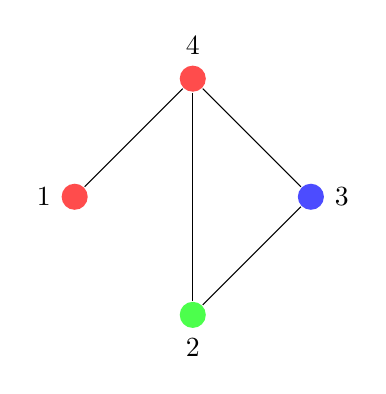
\begin{tikzpicture}
		   \begin{scope}
			   \node (0) at (0, 0)[pointred, label=180:1] {};
			   \node (1) at (1.5, 1.5)[pointred, label=90:4] {};
			   \node (2) at (3, 0)[pointblue, label=0:3] {};
			   \node (3) at (1.5, -1.5)[pointgreen, label=-90:2] {};
		   \end{scope}
		   \begin{scope}
			   \path [-] (0) edge (1);
			   \path [-] (1) edge (2);
			   \path [-] (1) edge (3);
			   \path [-] (2) edge (3);
		   \end{scope}
	   \end{tikzpicture}
	   \hspace{20pt}
	   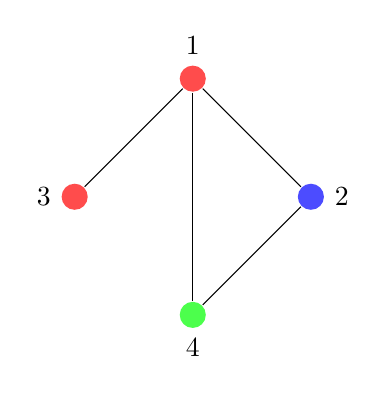
\begin{tikzpicture}
		   \begin{scope}
			   \node (0) at (0, 0)[pointred, label=180:3] {};
			   \node (1) at (1.5, 1.5)[pointred, label=90:1] {};
			   \node (2) at (3, 0)[pointblue, label=0:2] {};
			   \node (3) at (1.5, -1.5)[pointgreen, label=-90:4] {};
		   \end{scope}
		   \begin{scope}
			   \path [-] (0) edge (1);
			   \path [-] (1) edge (2);
			   \path [-] (1) edge (3);
			   \path [-] (2) edge (3);
		   \end{scope}
	   \end{tikzpicture}
	   \caption{Izomorfni grafovi $(G_1, \pi_1)$ i $(G_2, \pi_2)$.}
   \end{figure}

   \emph{Automorfizam} obojenog grafa $(G, \pi)$ je izomorfizam tog grafa sa
   samim sobom, odnosno $g \in S_n$ za koje važi $(G, \pi) = (G, \pi)^g$. Skup
   automorfizama grafa $(G, \pi)$ označavamo sa $Aut(G, \pi)$. Zajedno sa
   operacijom kompozicije preslikavanja skup $Aut(G, \pi)$ čini \emph{grupu
   automorfizama}.

   \begin{figure}[htp]
	   \label{img:aut}
	   \centering
	   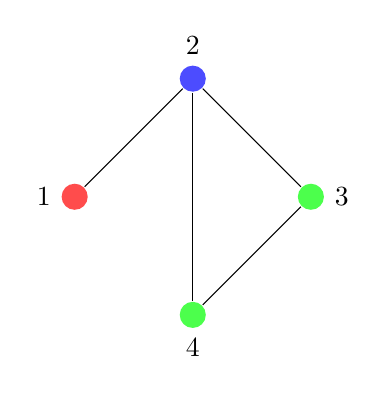
\begin{tikzpicture}
		   \begin{scope}
			   \node (0) at (0, 0)[pointred, label=180:1] {};
			   \node (1) at (1.5, 1.5)[pointblue, label=90:2] {};
			   \node (2) at (3, 0)[pointgreen, label=0:3] {};
			   \node (3) at (1.5, -1.5)[pointgreen, label=-90:4] {};
		   \end{scope}
		   \begin{scope}
			   \path [-] (0) edge (1);
			   \path [-] (1) edge (2);
			   \path [-] (1) edge (3);
			   \path [-] (2) edge (3);
		   \end{scope}
	   \end{tikzpicture}
	   \caption{Graf sa automorfizmom $g = (3\ 4)$.}
   \end{figure}


   \subsection{Kanonska forma}

   Neka je $f : \mathcal{G} \times \Pi \to S$ preslikavanje iz skupa svih
   obojenih grafova u proizvoljan skup $S$.  Kažemo da je $f$ \emph{funkcija
   invarijantna na imenovanje čvorova} ukoliko za svaki obojen graf $(G, \pi)$
   i svaku permutaciju $g \in S_n$ važi $f(G^g, \pi^g) = f(G, \pi)$.
   Neformalno, to znači da vrednost funkcije $f$ ne zavisi od konkretnog
   imenovanja čvorova grafa, već samo od njegove unutrašnje strukture.

   Ako na skupu $S$ postoji definisano dejstvo grupe $S_n$, kažemo da je $f$
   \emph{transformacija invarijantna na imenovanje čvorova} ukoliko za svaki
   obojen graf $(G, \pi)$ i svaku permutaciju $g \in S_n$ važi $f(G^g, \pi^g) =
   f(G, \pi)^g$.


   \begin{definition}
	   \emph{Kanonska forma} je preslikavanje $\mathcal{C} : \mathcal{G} \times \Pi \to
	   \mathcal{G} \times \Pi$ koje ispunjava sledeće uslove:
	   \begin{itemize}
		   \item[($\mathcal{C}1$)] Za svaki obojen graf $(G, \pi)$ važi
			   $\mathcal{C}(G, \pi) \cong (G,
			\pi)$
		\item[($\mathcal{C}2$)] $\mathcal{C}$ je funkcija invarijantna na
			imenovanje čvorova
	   \end{itemize}
   \end{definition}

   \begin{example}
	   Neka je definisano jedno totalno uređenje na skupu obojenih grafova,
	   recimo poređenjem njihovih binarnih reprezentacija $bin(G, \pi)$. Tada
	   je preslikavanje definisano sa $\mathcal{M}(G, \pi) = \max_{g \in S_n}
	   (G^g, \pi^g)$ kanonska forma.
   \end{example}


 \section{Stablo pretrage}

  Označimo sa $V^*$ skup svih konačnih nizova elemenata skupa $V$. Ako je $\nu
  \in V^*$ sa $|\nu|$ označavamo dužinu niza $\nu$. Ako je $\nu = (v_1, v_2,
  \dots, v_k) \in V^*$ i $w \in V$, onda $\nu \| w$ označava niz $(v_1, v_2,
  \dots, v_k, w)$. Za $0 \leq s \leq k$ prefiks niza $\nu$ dužine $s$ označavamo
  sa $[\nu]_s = (v_1, v_2, \dots, v_s)$. Uređenje $\leq$ na skupu $V^*$
  predstavlja leksikografski poredak.

  Čvorovi stabla pretrage  predstavljeni su nizovima elemenata skupa $V$, pri
  čemu korenu stabla odgovara prazan niz. U nastavku definišemo funkcije na
  osnovu kojih ćemo definisati pravila grananja u stablu.

  \begin{definition}
   \emph{Funkcija profinjavanja} je bilo koje preslikavanje $R : \mathcal{G}
	  \times \Pi \times V^* \to \Pi$ koje za svaki obojen graf $(G, \pi)$ i
	  svako $\nu \in V^*$ zadovoljava sledeće uslove:
  
   \begin{itemize}
       \item[(R1)] $R(G, \pi, \nu) \leq \pi$
       \item[(R2)] Ako je $v \in \nu$, onda je $\{v\}$ ćelija bojenja $R(G,
     	  \pi, \nu)$
       \item[(R3)] Za svako $g \in S_n$ važi $R(G^g, \pi^g, \nu^g) = R(G,
     	 \pi, \nu)^g$
   \end{itemize}
  \end{definition}

  \begin{definition}
   \emph{Funkcija odabira ciljne ćelije} je bilo koje preslikavanje $T :
	  \mathcal{G} \times \Pi \times V^* \to \mathcal{P}(V)$ koje za svaki
	  obojen graf $(G, \pi)$ i svako $\nu \in V^*$ zadovoljava sledeće
	  uslove:
  
   \begin{itemize}
       \item[(T1)] Ako je $R(G, \pi, \nu)$ diskretno, onda je $T(G, \pi, \nu) =
     	  \emptyset$
       \item[(T2)] Ako $R(G, \pi, \nu)$ nije diskretno, onda je $T(G, \pi, \nu)$
     	  nejedinična ćelija od $R(G, \pi, \nu)$
       \item[(T3)] Za svako $g \in S_n$ važi $T(G^g, \pi^g, \nu^g) = T(G, \pi,
     	 \nu)^g$
   \end{itemize}
  \end{definition}

  Kako je graf fiksan, ove funkcije možemo smatrati funkcijama čvorova stabla.
  Funkcija profinjavanja obezbeđuje postojanje bojenja pridruženog svakom čvoru
  stabla (koje postaje finije kako se spuštamo niz stablo). Funkcija odabira
  ciljne ćelije nam omogućava da odaberemo skup čvorova grafa koji nam služi za
  konstrukciju dece tog čvora u stablu. Treći uslov u obe definicije govori da
  su u pitanju transformacije invarijantne na imenovanje čvorova.

  \begin{definition}
      \emph{Stablo pretrage} $\mathcal{T}(G, \pi)$ određeno je sledećim uslovima:
  
   \begin{itemize}
       \item[($\mathcal{T}1$)] Koren stabla $\mathcal{T}(G, \pi)$ je prazan niz $()$
       \item[($\mathcal{T}2$)] Ako je $\nu$ čvor stabla $\mathcal{T}(G, \pi)$, njegova deca u
     	stablu su $\{$\nu$ \| w \mid w \in T(G, \pi, \nu)\}$
   \end{itemize}
  \end{definition}

  Iz definicije se vidi da je neki čvor list stabla ako i samo ako je njemu
  pridruženo bojenje diskretno. Primetimo da je ovako definisano stablo konačno
  zato što za svako $\nu$ koje je permutacija skupa $V$ važi da je bojenje
  pridruženo nekom njegovom prefiksu diskretno ili je njemu pridruženo bojenje
  diskretno.

  \begin{example}
	  Prikažimo jedno jednostavno stablo pretrage. Za funkciju odabira ciljne
	  ćelije možemo uzeti funkciju koja bira prvu nejediničnu ćeliju bojenja.
	  Za funkciju profinjavanja možemo uzeti funkciju koja dodeljuje boje
	  čvorovima u skladu sa početnim bojenjem $\pi$, pri čemu čvorove niza
	  $\nu$ izdvaja u zasebne ćelije. Na slici \ref{img:tree} je prikazano
	  stablo pretrage jednog grafa.
  \end{example}

   \begin{figure}[htp]
	   \label{img:tree}
	   \centering
	   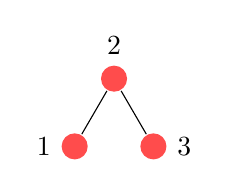
\begin{tikzpicture}
		   \begin{scope}
			   \node (1) at (0, 0)[pointred, label=180:1] {};
			   \node (2) at (0.5, 0.86)[pointred, label=90:2] {};
			   \node (3) at (1, 0)[pointred, label=0:3] {};
		   \end{scope}
		   \begin{scope}
			   \path [-] (1) edge (2);
			   \path [-] (2) edge (3);
		   \end{scope}
	   \end{tikzpicture}

	   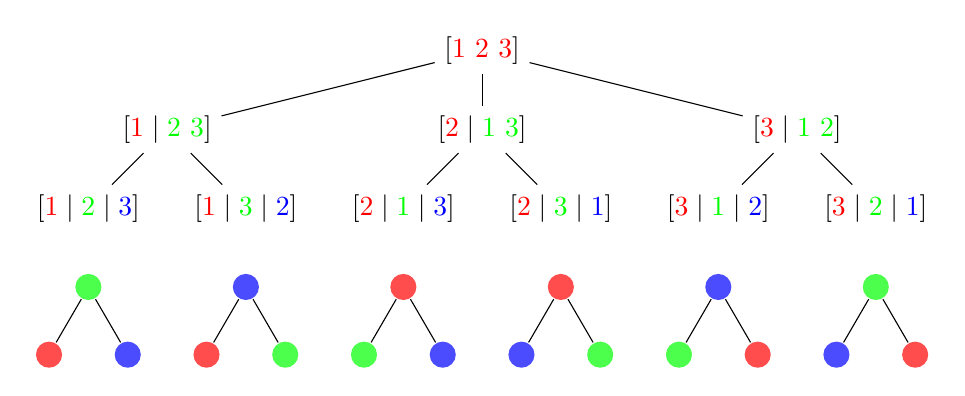
\begin{tikzpicture}
		   \begin{scope}
			   \node (0) at (0, 0) {$[{\color{red}1\ 2\ 3}]$};
			   \node (1) at (-4, -1) {$[{\color{red}1} \mid {\color{green}2\ 3}]$};
			   \node (2) at (0, -1) {$[{\color{red}2} \mid {\color{green}1\ 3}]$};
			   \node (3) at (4, -1) {$[{\color{red}3} \mid {\color{green}1\ 2}]$};
			   \node (12) at (-5, -2) {$[{\color{red}1} \mid {\color{green}2} \mid {\color{blue}3}]$};
			   \node (13) at (-3, -2) {$[{\color{red}1} \mid {\color{green}3} \mid {\color{blue}2}]$};
			   \node (21) at (-1, -2) {$[{\color{red}2} \mid {\color{green}1} \mid {\color{blue}3}]$};
			   \node (23) at (1, -2) {$[{\color{red}2} \mid {\color{green}3} \mid {\color{blue}1}]$};
			   \node (31) at (3, -2) {$[{\color{red}3} \mid {\color{green}1} \mid {\color{blue}2}]$};
			   \node (32) at (5, -2) {$[{\color{red}3} \mid {\color{green}2} \mid {\color{blue}1}]$};

			   \node (a1) at (-5.5, -3.86)[pointred] {};
			   \node (a2) at (-5, -3)[pointgreen] {};
			   \node (a3) at (-4.5, -3.86)[pointblue] {};

			   \node (b1) at (-3.5, -3.86)[pointred] {};
			   \node (b2) at (-3, -3)[pointblue] {};
			   \node (b3) at (-2.5, -3.86)[pointgreen] {};

			   \node (c1) at (-1.5, -3.86)[pointgreen] {};
			   \node (c2) at (-1, -3)[pointred] {};
			   \node (c3) at (-0.5, -3.86)[pointblue] {};

			   \node (d1) at (0.5, -3.86)[pointblue] {};
			   \node (d2) at (1, -3)[pointred] {};
			   \node (d3) at (1.5, -3.86)[pointgreen] {};

			   \node (e1) at (2.5, -3.86)[pointgreen] {};
			   \node (e2) at (3, -3)[pointblue] {};
			   \node (e3) at (3.5, -3.86)[pointred] {};

			   \node (f1) at (4.5, -3.86)[pointblue] {};
			   \node (f2) at (5, -3)[pointgreen] {};
			   \node (f3) at (5.5, -3.86)[pointred] {};
		   \end{scope}
		   \begin{scope}
			   \path [-] (0) edge (1);
			   \path [-] (0) edge (2);
			   \path [-] (0) edge (3);
			   \path [-] (1) edge (12);
			   \path [-] (1) edge (13);
			   \path [-] (2) edge (21);
			   \path [-] (2) edge (23);
			   \path [-] (3) edge (31);
			   \path [-] (3) edge (32);

			   \path [-] (a1) edge (a2);
			   \path [-] (a2) edge (a3);

			   \path [-] (b1) edge (b2);
			   \path [-] (b2) edge (b3);

			   \path [-] (c1) edge (c2);
			   \path [-] (c2) edge (c3);

			   \path [-] (d1) edge (d2);
			   \path [-] (d2) edge (d3);

			   \path [-] (e1) edge (e2);
			   \path [-] (e2) edge (e3);

			   \path [-] (f1) edge (f2);
			   \path [-] (f2) edge (f3);
		   \end{scope}
	   \end{tikzpicture}
	   \caption{Stablo pretrage koje generiše sve permutacije skupa čvorova.}
   \end{figure}

  Dejstvo grupe $S_n$ na stablo definiše se slično kao za bilo koju drugu
  strukturu. Naredna lema pokazuje da je ovako definisano stablo invarijantno na
  imenovanje čvorova grafa.

  \begin{lemma}
      Za svaki obojen graf $(G, \pi)$ i svako $g \in S_n$ važi
      $\mathcal{T}(G^g, \pi^g) = \mathcal{T}(G, \pi)^g$.
  \end{lemma}

  \begin{proof}
      Dokažimo da za svaki čvor $\nu$ stabla $\mathcal{T}(G, \pi)$ važi da je
      $\nu^g$ čvor stabla $\mathcal{T}(G^g, \pi^g)$. Dokaz izvodimo indukcijom
      po strukturi stabla.
      \begin{itemize}
     	 \item[] \textbf{Baza indukcije} Prazan niz je koren stabla
     		 $\mathcal{T}(G^g, \pi^g)$, pa tvrđenje trivijalno važi.
     	 \item[] \textbf{Induktivni korak} Pretpostavimo da tvrđenje važi za
     		 čvor $\nu$. Neka je $\nu \| w$ dete čvora $\nu$ za neko $w \in
     		 T(G, \pi, \nu)$. Tada je $(\nu \| w)^g = \nu^g \| w^g$, ali kako
     		 važi $w^g \in T(G, \pi, \nu)^g =_{(T3)} T(G^g, \pi^g, \nu^g)$
     		 to je $\nu^g \| w^g$ dete čvora $\nu^g$ u stablu $\mathcal{T}(G^g,
     		 \pi^g)$.
      \end{itemize}
      Time smo dokazali da je stablo $\mathcal{T}(G, \pi)^g$ podstablo od
      $\mathcal{T}(G^g, \pi^g)$ ($\mathcal{T}(G, \pi)^g \subseteq
      \mathcal{T}(G^g, \pi^g)$). Prema prethodno dokazanom važi
      $\mathcal{T}(G^g, \pi^g)^{g^{-1}} \subseteq \mathcal{T}(G, \pi)$, pa
      primenom $g$ na obe strane konačno dobijamo $\mathcal{T}(G^g, \pi^g)
      \subseteq \mathcal{T}(G, \pi)^g$.
  \end{proof}

  \begin{corrolary}
	  \label{corr:auttree}
      Neka je $\nu$ čvor stabla $\mathcal{T}(G, \pi)$ i neka $\mathcal{T}(G,
      \pi, \nu)$ označava njegovo podstablo sa korenom u $\nu$. Ako je $g
      \in Aut(G, \pi)$, onda je $\nu^g$ čvor stabla $\mathcal{T}(G, \pi)$ i
      važi $\mathcal{T}(G, \pi, \nu^g) = \mathcal{T}(G, \pi, \nu)^g$.
  \end{corrolary}

  \begin{lemma}
	  Neka je $\nu$ čvor stabla $\mathcal{T}(G, \pi)$ i $\pi_\nu = R(G, \pi,
	  \nu)$. Tada je grupa automorfizama obojenog grafa $(G, \pi_\nu)$ jednaka
	  stabilizatoru niza $\nu$ u grupi automorfizama grafa $(G, \pi)$, odnosno
	  $Aut(G, \pi_\nu) = \Sigma_\nu^{Aut(G, \pi)}$.
  \end{lemma}

  \begin{proof}
	  Neka je $g \in Aut(G, \pi_\nu)$. Tada je $\pi_\nu^g = \pi_\nu$, pa za
	  svako $v$ važi $\pi_\nu^g(v) = \pi_\nu(v)$. Na osnovu uslova $(R2)$ za $v
	  \in \nu$ važi $\{v\} = \pi_\nu^{-1}(\pi_\nu(v)) =
	  \pi_\nu^{-1}(\pi_\nu^g(v)) = \pi_\nu^{-1}(\pi_\nu(g^{-1}v)) \ni g^{-1}v$
	  odakle sledi $v^g = v$, odnosno $g$ stabilizuje svako $v \in \nu$.

	  Sa druge strane, neka $g \in Aut(G, \pi)$ stabilizuje $\nu$. Tada po (R3)
	  važi $\pi_\nu^g = R(G, \pi, \nu)^g = R(G^g, \pi^g, \nu^g) = R(G, \pi,
	  \nu) = \pi_\nu$, pa je $g \in Aut(G, \pi_\nu)$.
  \end{proof}

 \section{Invarijanta stabla}

  \begin{definition}
	  \emph{Invarijanta stabla} je preslikavanje $\phi : \mathcal{G} \times \Pi
	  \times V^* \to F$ za neki potpuno uređen skup $F$ koje za sve obojene
	  grafove $(G, \pi)$ i različite čvorove $\nu_1, \nu_2 \in \mathcal{T}(G,
	  \pi)$ ispunjava sledeće uslove:

	  \begin{itemize}
		  \item[(\phi1)] Ako su $\nu_1, \nu_2 \in \mathcal{T}(G, \pi)$ takvi
			  da je $|\nu_1|=|\nu_2|$ i $\phi(G, \pi, \nu_1) < \phi(G,
			  \phi_0, \nu_2)$, onda za sve $\omega_1 \in \mathcal{T}(G, \pi,
			  \nu_1)$ i $\omega_2 \in \mathcal{T}(G, \pi, \nu_2)$ važi
			  $\phi(G, \pi, \omega_1) < \phi(G, \pi, \omega_2)$
		  \item[(\phi2)] Ako su $\nu_1, \nu_2 \in \mathcal{T}(G, \pi)$ takvi
			  da su $\pi_1 = R(G, \pi, \nu_1)$ i $\pi_2 = R(G, \pi, \nu_2)$
			  diskretna bojenja, onda je $\phi(G, \pi, \nu_1) = \phi(G,
			  \pi, \nu_2) \implies G^{\pi_1} = G^{\pi_2}$
		  \item[(\phi3)] $\phi$ je funkcija invarijantna na imenovanje čvorova
			  grafa
	  \end{itemize}

	  Listovi $\nu_1$ i $\nu_2$ su \emph{ekvivalentni} ako i samo ako $\phi(G,
	  \pi, \nu_1) = \phi(G, \pi, \nu_2)$.
  \end{definition}

  \begin{example}
	  Definišimo $\phi(G, \pi, \nu)$ koristeći pomoćnu funkciju $f$ kao niz
	  vrednosti $(f(G, \pi, [\nu]_0), f(G, \pi, [\nu]_1), \dots, f(G, \pi,
	  [\nu]_{|\nu|}))$, pri čemu u slučaju da je $\nu$ list možemo na taj niz
	  nadovezati i binarnu reprezentaciju grafa permutovanog bojenjem $R(G, \pi,
	  \nu)$. Ovako definisano $\phi$ ispunjava uslove ($\phi$1-2). Ako za
	  pomoćnu funkciju $f$ odaberemo npr. proizvod zbirova stepena čvorova
	  ćelija, dobijamo jednu jednostavnu invarijantu stabla. Vrednosti
	  invarijante stabla iz primera \ref{img:tree} prikazane su na slici
	  \ref{img:invariant}.
  \end{example}

   \begin{figure}[htp]
	   \label{img:invariant}
	   \centering
	   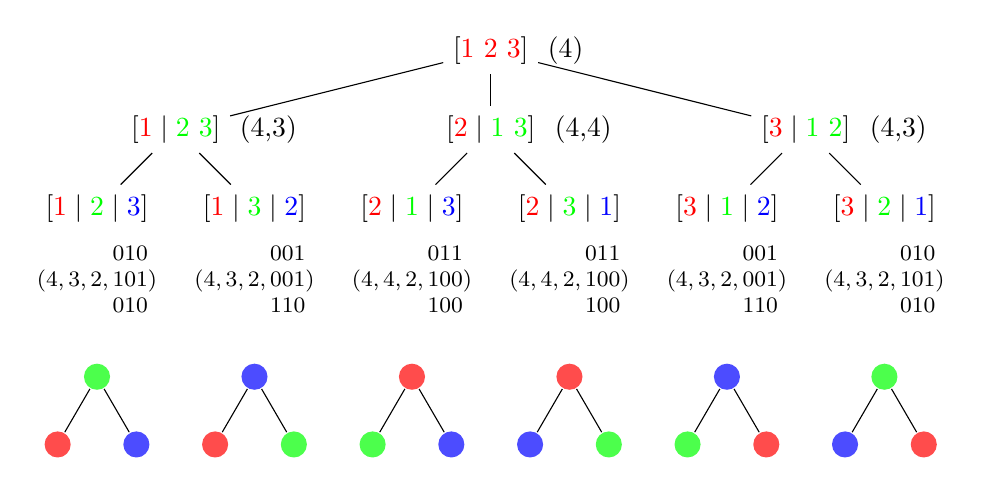
\begin{tikzpicture}
		   \begin{scope}
			   \node (0) at (0, 0) [label=0:{(4)}] {$[{\color{red}1\ 2\ 3}]$};
			   \node (1) at (-4, -1) [label=0:{(4,3)}] {$[{\color{red}1} \mid {\color{green}2\ 3}]$};
			   \node (2) at (0, -1) [label=0:{(4,4)}] {$[{\color{red}2} \mid {\color{green}1\ 3}]$};
			   \node (3) at (4, -1) [label=0:{(4,3)}] {$[{\color{red}3} \mid {\color{green}1\ 2}]$};
			   \node (12) at (-5, -2) [label=270:{\footnotesize $(4,3,2,\begin{matrix}010\\101\\010\end{matrix})$}] {$[{\color{red}1} \mid {\color{green}2} \mid {\color{blue}3}]$};
			   \node (13) at (-3, -2) [label=270:{\footnotesize $(4,3,2,\begin{matrix}001\\001\\110\end{matrix})$}] {$[{\color{red}1} \mid {\color{green}3} \mid {\color{blue}2}]$};
			   \node (21) at (-1, -2) [label=270:{\footnotesize $(4,4,2,\begin{matrix}011\\100\\100\end{matrix})$}] {$[{\color{red}2} \mid {\color{green}1} \mid {\color{blue}3}]$};
			   \node (23) at (1, -2) [label=270:{\footnotesize $(4,4,2,\begin{matrix}011\\100\\100\end{matrix})$}] {$[{\color{red}2} \mid {\color{green}3} \mid {\color{blue}1}]$};
			   \node (31) at (3, -2) [label=270:{\footnotesize $(4,3,2,\begin{matrix}001\\001\\110\end{matrix})$}] {$[{\color{red}3} \mid {\color{green}1} \mid {\color{blue}2}]$};
			   \node (32) at (5, -2) [label=270:{\footnotesize $(4,3,2,\begin{matrix}010\\101\\010\end{matrix})$}] {$[{\color{red}3} \mid {\color{green}2} \mid {\color{blue}1}]$};

			   \node (a1) at (-5.5, -5)[pointred] {};
			   \node (a2) at (-5, -4.14)[pointgreen] {};
			   \node (a3) at (-4.5, -5)[pointblue] {};

			   \node (b1) at (-3.5, -5) [pointred] {};
			   \node (b2) at (-3, -4.14)[pointblue] {};
			   \node (b3) at (-2.5, -5)[pointgreen] {};

			   \node (c1) at (-1.5, -5)[pointgreen] {};
			   \node (c2) at (-1, -4.14)[pointred] {};
			   \node (c3) at (-0.5, -5)[pointblue] {};

			   \node (d1) at (0.5, -5)[pointblue] {};
			   \node (d2) at (1, -4.14)[pointred] {};
			   \node (d3) at (1.5, -5)[pointgreen] {};

			   \node (e1) at (2.5, -5)[pointgreen] {};
			   \node (e2) at (3, -4.14)[pointblue] {};
			   \node (e3) at (3.5, -5)[pointred] {};

			   \node (f1) at (4.5, -5)[pointblue] {};
			   \node (f2) at (5, -4.14)[pointgreen] {};
			   \node (f3) at (5.5, -5)[pointred] {};
		   \end{scope}
		   \begin{scope}
			   \path [-] (0) edge (1);
			   \path [-] (0) edge (2);
			   \path [-] (0) edge (3);
			   \path [-] (1) edge (12);
			   \path [-] (1) edge (13);
			   \path [-] (2) edge (21);
			   \path [-] (2) edge (23);
			   \path [-] (3) edge (31);
			   \path [-] (3) edge (32);

			   \path [-] (a1) edge (a2);
			   \path [-] (a2) edge (a3);

			   \path [-] (b1) edge (b2);
			   \path [-] (b2) edge (b3);

			   \path [-] (c1) edge (c2);
			   \path [-] (c2) edge (c3);

			   \path [-] (d1) edge (d2);
			   \path [-] (d2) edge (d3);

			   \path [-] (e1) edge (e2);
			   \path [-] (e2) edge (e3);

			   \path [-] (f1) edge (f2);
			   \path [-] (f2) edge (f3);
		   \end{scope}
	   \end{tikzpicture}
   \caption{Invarijanta stabla.}
   \end{figure}


  U nastavku ćemo kroz dve teoreme prikazati značaj ovako definisane
  invarijante stabla. Označimo za proizvoljan čvor stabla $\nu$ njegovo bojenje
  dobijeno funkcijom profinjavanja sa $\pi_\nu = R(G, \pi, \nu)$. 

  \begin{lemma}
	  \label{lemma:autequiv}
	  Neka je $g \in Aut(G, \pi)$ i listovi $\nu_1$ i $\nu_2$ takvi da je
	  $\nu_1^g = \nu_2$. Tada su $\nu_1$ i $\nu_2$ ekvivalentni i $g =
	  \pi_{\nu_2}^{-1}\pi_{\nu_1}$.
  \end{lemma}

  \begin{proof}
	  Na osnovu svojstva ($\phi3$) invarijante stabla i činjenice da je $g$
	  automorfizam sledi $\phi(G, \pi, \nu_1) =_{(\phi_3)} \phi(G^g, \pi^g,
	  \nu_1^g) =_{g \in Aut(G, \pi)} \phi(G, \pi, \nu_1^g) = \phi(G, \pi,
	  \nu_2)$, odnosno $\nu_1$ i $\nu_2$ su ekvivalentni. Dalje, važi
	  $\pi_{\nu_2}^{-1}\pi_{\nu_1} = \pi_{\nu_1^g}^{-1}\pi_{\nu_1} =_{(R3)}
	  (\pi_{\nu_1}^g)^{-1}\pi_{\nu_1} = (\pi_{\nu_1} g^{-1})^{-1} \pi_{\nu_1} = g
	  \pi_{\nu_1}^{-1} \pi_{\nu_1} = g$.
  \end{proof}

  \begin{lemma}
	  Neka su $\alpha$ i $\beta$ diskretna bojenja finija od bojenja $\pi$.
	  Tada je $\pi^\alpha = \pi^\beta$.
  \end{lemma}

  \begin{proof}
	  Dokaz izvodimo nizom sitnih tvrđenja.

	  \begin{enumerate}
		  \item $id \leq \pi^\alpha$

			  Neka su $x$ i $y$ proizvoljni. Važi $\pi^\alpha(x) <
			  \pi^\alpha(y) \iff \pi(\alpha^{-1}(x)) < \pi(\alpha^{-1}(y))$, pa
			  kako je $\alpha \leq \pi$ sledi $\alpha(\alpha^{-1}(x)) <
			  \alpha(\alpha^{-1}(y))$ odnosno $x < y$. Kontrapozicijom dobijamo
			  i $x \leq y \implies \pi^\alpha(x) \leq \pi^\alpha(y)$.

		  \item $(\pi^\alpha)^{-1}(c) = [n, m]$ za neko $n, m \in \mathbb{N}$
			  gde je $[n, m] = \{k \in \mathbb{N} \mid n \leq k \leq m\}$

			  Za svako $x, y, z $ važi $x \leq y \leq z \implies \pi^\alpha(x)
			  \leq \pi^\alpha(y) \leq \pi^\alpha(z)$, pa ako je $\pi^\alpha(x)
			  = \pi^\alpha(z) = c$, onda je i $\pi^\alpha(y) = c$.

		  \item $\pi^\alpha(n + 1) = \pi^\alpha(n)$ ili $\pi^\alpha(n+1) =
			  \pi^\alpha(n) + 1$

			  Neka je $\pi^\alpha(n+1) \neq \pi^\alpha(n)$. Tada je $n + 1 \geq
			  n \implies \pi^\alpha(n+1) \geq \pi^\alpha(n)$, pa je
			  $\pi^\alpha(n+1) > \pi^\alpha(n)$ jer su po pretpostavci
			  različiti. Pretpostavimo da je $\pi^\alpha(n+1) > \pi^\alpha(n) +
			  1$. Tada postoji $m$ takvo da je $\pi^\alpha(m) = \pi^\alpha(n) +
			  1$, ali iz $\pi^\alpha(n) < \pi^\alpha(m) < \pi^\alpha(n+1)
			  \implies n < m < n + 1$ sledi kontradikcija.

		  \item $|(\pi^\alpha)^{-1}(c)| = |\pi^{-1}(c)|$

			  Važi da je $(\pi^\alpha)^{-1}(c) = \{m \mid \pi^\alpha(m) = c\} =
			  \{m^\alpha \mid \pi^\alpha(m^\alpha) = c\} = \{m^\alpha \mid
			  \pi(m) = c\} = \pi^{-1}(c)^\alpha$. Odatle je
			  $|(\pi^\alpha)^{-1}(c)| = |\pi^{-1}(c)^\alpha| = |\pi^{-1}(c)|$.

		  \item $(\pi^\alpha)^{-1}(c) = (\pi^\beta)^{-1}(c)$

			  Dokaz izvodimo indukcijom po $c$.

			  \begin{itemize}
				  \item[] \textbf{Baza indukcije} Kako je $1 \leq x$ za sve
					  $x$, onda iz $id \leq \pi^\alpha$ sledi $\pi^\alpha(1)
					  \leq \pi^\alpha(x)$ za sve $x$ pa je $\pi^\alpha(1) = 1$.
					  Dalje, kako je $|(\pi^\alpha)^{-1}(1)| = |\pi^{-1}(1)|$,
					  mora važiti $(\pi^\alpha)^{-1}(1) = [1, |\pi^{-1}(1)|]$.
					  Analogno se pokazuje i za $\beta$.

				  \item[] \textbf{Induktivni korak} Neka je po induktivnoj
					  pretpostavci $(\pi^\alpha)^{-1}(c) = (\pi^\beta)^{-1}(c)
					  = [n, m]$. Tada je $\pi^\alpha(m+1) \neq \pi^\alpha(m)$,
					  pa je $\pi^\alpha(m+1) = \pi^\alpha(m) + 1$ i $m+1$ je
					  najmanje u $(\pi^\alpha)^{-1}(c+1)$. Odatle važi
					  $(\pi^\alpha)^{-1}(c+1) = [m + 1, m + |\pi^{-1}(c+1)|]$.
					  Analogno se pokazuje i za $\beta$.
			  \end{itemize}
	  \end{enumerate}
  \end{proof}

  \begin{theorem}
	  \label{thm:aut}
	  Za svaki list $\nu$ važi $Aut(G, \pi) = \{\pi_{\omega}^{-1}\pi_{\nu}
	  \mid \text{$\nu$ i $\omega$ su ekvivalentni} \}$.
  \end{theorem}
  
  \begin{proof}
	  Neka je $g \in Aut(G, \pi)$. Tada je po posledici \ref{corr:auttree}
	  $\nu^g$ list stabla $\mathcal{T}(G, \pi)$. Po prethodno dokazanoj lemi
	  \ref{lemma:autequiv} su $\nu$ i $\nu^g$ ekvivalentni i $g =
	  \pi_{\nu^g}^{-1}\pi_\nu$ što je element skupa sa desne strane jednakosti.
	  Sa druge strane, ako su $\nu$ i $\omega$ ekvivalentni, onda je
	  $G^{\pi_\nu} = G^{\pi_\omega}$, pa je $\pi_\omega^{-1}\pi_\nu \in Aut(G,
	  \pi)$.
  \end{proof}

	Prethodna teorema pokazuje da je otkrivanjem svih čvorova ekvivalentnih
	jednom čvoru moguće odrediti grupu automorfizama datog grafa. Naravno,
	ovakav način određivanja grupe automorfizama nije veoma efikasan pošto se
	grupa generiše član po član. Ovo se može poboljšati odsecanjem pretrage o
	čemu će biti reči u narednom odeljku.
	
	\begin{example}
		Posmatrajmo prvi list stabla sa slike \ref{img:invariant}. Na osnovu
		prethodne teoreme je moguće odrediti skup svih automorfizama grafa.
		Kako je taj list ekvivalentan samom sebi, $id \in Aut(G, \pi)$.  Kako
		je ekvivalentan poslednjem listu stabla, $(1\ 3) \in Aut(G, \pi)$. Ne
		postoje drugi automorfizmi jer ne postoje drugi listovi ekvivalentni
		prvom listu stabla, pa je $Aut(G, \pi) = \{id, (1\ 3)\}$.
	\end{example}

  \begin{definition}
	  Neka je $\nu^*$ list stabla $\mathcal{T}(G, \pi)$ u kom invarijanta
	  $\phi(G, \pi, \nu)$ dostiže maksimum. \emph{Kanonska forma} obojenog
	  grafa $(G, \pi)$ je funkcija $\mathcal{C}(G, \pi) = (G,
	  \pi)^{\pi_{\nu^*}}$.
  \end{definition}

  Primetimo da zbog uslova $(\phi2)$ definicija ne zavisi od izbora lista
  $\nu^*$. Naredna teorema opravdava naziv i oznaku funkcije.

  \begin{theorem}
	  Funkcija $\mathcal{C}(G, \pi)$ je kanonska forma.
  \end{theorem}

  \begin{proof}
		Dokazujemo da ovako definisana funkcija ispunjava uslove kanonske forme za
		svaki obojen graf $(G, \pi)$.
	  \begin{itemize}
		  \item [($\mathcal{C}1$)] Kako je $\mathcal{C}(G, \pi) = (G,
			  \pi)^{\pi_{\nu^*}}$ to je $\mathcal{C}(G, \pi) \cong (G, \pi)$ za
			  izomorfizam $\pi_{\nu^*}$.
		  \item [($\mathcal{C}2$)] Za svako $g \in S_n$ i svako $\nu \in
			  \mathcal{T}(G, \pi)$ važi $\nu^g \in \mathcal{T}(G, \pi)^g =
			  \mathcal{T}(G^g, \pi^g)$ kao i $\phi(G^g, \pi^g, \nu^g) = \phi(G,
			  \pi, \nu)$, pa je $\nu^*^g$ list u kom invarijanta stabla
			  $\mathcal{T}(G^g, \pi^g)$ dostiže maksimalnu vrednost.  Odatle
			  sledi $\mathcal{C}(G^g, \pi^g) = (G^g, \pi^g)^{R(G^g, \pi^g,
			  \nu^*^g)} = (G^g, \pi^g)^{\pi_{v^*}^g} = (G, \pi)^{\pi_{v^*}} =
			  \mathcal{C}(G, \pi)$ pa je $\mathcal{C}$ funkcija invarijantna na
			  imenovanje čvorova.
	  \end{itemize}
  \end{proof}

	\begin{example}
		Posmatrajmo stablo sa slike \ref{img:invariant}. Na osnovu prethodne
		teoreme je moguće odrediti kanonsku formu grafa. U pitanju je graf koji
		se dobija bilo kojom od permutacija $(2\ 1)$ ili $(3\ 2\ 1)$ jer su to
		permutacije sa najvećom invarijantnom u stablu.
	\end{example}

 \section{Odsecanje pretrage}

  Stablo pretrage može biti veoma veliko, pa pretraga kompletnog stabla nije
  poželjna. To možemo rešiti uvođenjem tri različite operacije odsecanja.
  \begin{itemize}
	  \item Neka su $\nu_1$ i $\nu_2$ različiti čvorovi stabla $\mathcal{T}(G,
		  \pi)$ takvi da je $|\nu_1|=|\nu_2|$ i $\phi(G, \pi, \nu_1) >
		  \phi(G, \pi, \nu_2)$. Operacija $P_A(\nu_1, \nu_2)$ podrazumeva
		  odsecanje podstabla $\mathcal{T}(G, \pi, \nu_2)$.
	  \item Neka su $\nu_1$ i $\nu_2$ različiti čvorovi stabla $\mathcal{T}(G,
		  \pi)$ takvi da je $|\nu_1|=|\nu_2|$ i $\phi(G, \pi, \nu_1) \neq
		  \phi(G, \pi, \nu_2)$. Operacija $P_B(\nu_1, \nu_2)$ podrazumeva
		  odsecanje podstabla $\mathcal{T}(G, \pi, \nu_2)$.
	  \item Neka su $\nu_1$ i $\nu_2$ različiti čvorovi stabla $\mathcal{T}(G,
		  \pi)$ takvi da je $\nu_1 < \nu_2$ i $\nu_1^g=\nu_2$ za neko $g \in
		  Aut(G, \pi)$. Operacija $P_C(\nu_1, g)$ podrazumeva odsecanje
		  podstabla $\mathcal{T}(G, \pi, \nu_2)$.
  \end{itemize}

  Operacije $P_A$ i $P_C$ su definisane tako da očuvavaju mogućnost određivanja
  kanonske forme u stablu. Slično, operacije $P_B$ i $P_C$ očuvavaju mogućnost
  određivanja grupe automorfizama na osnovu stabla. Naredna teorema opravdava
  uvođenje ovih operacija i pokazuje da one ne narušavaju rezultate teorema o
  određivanju grupe automorfizama i kanonske forme.

  \begin{theorem}
	  Neka je $(G, \pi)$ obojen graf.
	  \begin{enumerate}
		  \item Neka je nad stablom $\mathcal{T}(G, \pi)$ izvršen proizvoljan
			  niz operacija $P_A$ i $P_C$. Tada u dobijenom stablu postoji bar
			  jedan list $\nu$ takav da je $\phi(G, \pi, \nu) = \phi(G, \pi,
			  \nu^*)$.
		  \item Neka je $\nu_0$ list stabla $\mathcal{T}(G, \pi)$ i neka je nad
			  stablom izvršen proizvoljan niz operacija $P_B(\nu_1, \nu_2)$ i
			  $P_C$ gde je $\phi(G, \pi, \nu_2) \neq \phi(G, \pi,
			  [\nu_0]_{s})$ za sve $0 \leq s \leq |\nu_0|$ i neka su $g_1,
			  \dots, g_k$ svi automorfizmi korišćeni u izvršenim operacijama
			  $P_C$.  Tada je grupa automorfizama $Aut(G, \pi)$ generisana
			  skupom $\{g_1, \dots, g_k\} \cup \{g \in Aut(G, \pi) \mid \nu_0^g
			  \text{ nije uklonjen}\}$.
	  \end{enumerate}
  \end{theorem}

  \begin{proof}
	  Dokažimo za početak nekoliko pomoćnih tvrđenja.

	  Nijedna operacija $P_A$ ne uklanja listove u kojima je vrednost
	  invarijante maksimalna. Pretpostavimo suprotno. Neka je $\nu_1$ list u
	  kom invarijanta stabla dostiže maksimum i neka je $\nu'_1$ predak od
	  $\nu_1$. Operacija $P_A(\nu'_2, \nu'_1)$ uklanja $\nu'_1$ ako je $\phi(G,
	  \pi, \nu'_1) < \phi(G, \pi, \nu'_2)$, pa po svojstvu $(\phi1)$ za
	  proizvoljan list $\nu_2$ u $\mathcal{T}(G, \pi, \nu'_2)$ važi $\phi(G,
	  \pi, \nu_1) < \phi(G, \pi, \nu_2)$, što je u kontradikciji sa
	  pretpostavkom da je vrednost invarijante maksimalna u $\nu_1$.

	  Nijedna operacija $P_B$ ne uklanja nijedan list $\nu$ ekvivalentan listu
	  $\nu_0$ (iz drugog dela teoreme). Iz pretpostavke teoreme nijedna
	  operacija $P_B(\nu_1, \nu_2)$ ne uklanja čvor $\nu_2$ takav da je
	  $\phi(G, \pi, [\nu_0]_{|\nu_2|}) = \phi(G, \pi, \nu_2)$, pa samim tim ne
	  uklanja nijedan čvor $[\nu]_{s}$ za $0 \leq s \leq |\nu|$.

	  Nijedna operacija $P_C$ ne uklanja leksikografski najmanji među
	  ekvivalentnim listovima. Štaviše, nijedna operacija $P_C$ ne uklanja
	  leksikografski najmanji čvor iz $\Omega_\nu^{<g_1, \dots, g_k>}$ za bilo
	  koje $\nu$. Neka je bez umanjenja opštosti $\nu$ leksikografski najmanji
	  list u svojoj orbiti. Operacija $P_C(\omega, g)$ uklanja čvor $\omega^g$
	  ako je $\omega < \omega^g$, pa je $[\nu]_{|\omega|} \neq \omega^g$ pošto
	  je ili $[\nu]_{|\omega|} < \omega$ ili su $\omega$ i $[\nu]_{|\omega|}$ iz
	  različitih orbita.
	  \begin{enumerate}
		  \item Na osnovu dokazanih svojstava operacija $P_A$ i $P_C$ iz stabla
			  se ne uklanja leksikografski najmanji list $\nu$ ekvivalentan
			  listu $\nu^*$.
		  \item Ako je $g \in Aut(G, \pi)$, onda na osnovu dokazanih svojstva
			  operacija $P_B$ i $P_C$ važi da iz stabla nije uklonjen
			  leksikografski najmanji list oblika $\nu_0^{hg}$ za neko $h \in <
			  \negmedspace g_1, \dots, g_k \negmedspace >$, izborom $\omega =
			  \nu_0^g$. Odatle sledi da je $hg \in < \negmedspace \{g_1, \dots,
			  g_k\} \cup \{g \in Aut(G, \pi) \mid \nu_0^g \text{ nije
			  uklonjen}\} \negmedspace >$, pa je i $g$ element generisane
			  grupe.
	  \end{enumerate}
  \end{proof}

   \begin{figure}[htp]
	   \label{img:prune}
	   \centering
	   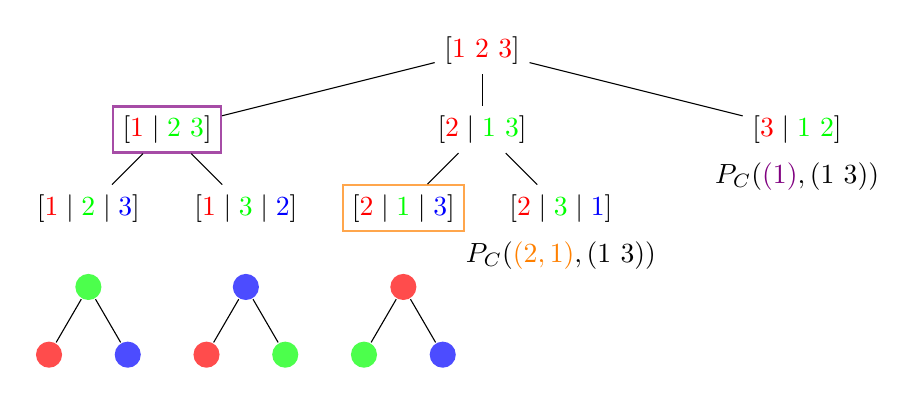
\begin{tikzpicture}
		   \begin{scope}
			   \node (0) at (0, 0)  {$[{\color{red}1\ 2\ 3}]$};
			   \node (1) at (-4, -1) [rectangle, draw=violet!70, thick] {$[{\color{red}1} \mid {\color{green}2\ 3}]$};
			   \node (2) at (0, -1)  {$[{\color{red}2} \mid {\color{green}1\ 3}]$};
			   \node (3) at (4, -1) [label=270:{$P_C({\color{violet}(1)}, (1\ 3))$}] {$[{\color{red}3} \mid {\color{green}1\ 2}]$};
			   \node (12) at (-5, -2)  {$[{\color{red}1} \mid {\color{green}2} \mid {\color{blue}3}]$};
			   \node (13) at (-3, -2)  {$[{\color{red}1} \mid {\color{green}3} \mid {\color{blue}2}]$};
			   \node (21) at (-1, -2) [rectangle,draw=orange!70,thick] {$[{\color{red}2} \mid {\color{green}1} \mid {\color{blue}3}]$};
			   \node (23) at (1, -2) [label=270:{$P_C({\color{orange}(2,1)}, (1\ 3)) $}] {$[{\color{red}2} \mid {\color{green}3} \mid {\color{blue}1}]$};

			   \node (a1) at (-5.5, -3.86)[pointred] {};
			   \node (a2) at (-5, -3)[pointgreen] {};
			   \node (a3) at (-4.5, -3.86)[pointblue] {};

			   \node (b1) at (-3.5, -3.86)[pointred] {};
			   \node (b2) at (-3, -3)[pointblue] {};
			   \node (b3) at (-2.5, -3.86)[pointgreen] {};

			   \node (c1) at (-1.5, -3.86)[pointgreen] {};
			   \node (c2) at (-1, -3)[pointred] {};
			   \node (c3) at (-0.5, -3.86)[pointblue] {};
		   \end{scope}
		   \begin{scope}
			   \path [-] (0) edge (1);
			   \path [-] (0) edge (2);
			   \path [-] (0) edge (3);
			   \path [-] (1) edge (12);
			   \path [-] (1) edge (13);
			   \path [-] (2) edge (21);
			   \path [-] (2) edge (23);

			   \path [-] (a1) edge (a2);
			   \path [-] (a2) edge (a3);

			   \path [-] (b1) edge (b2);
			   \path [-] (b2) edge (b3);

			   \path [-] (c1) edge (c2);
			   \path [-] (c2) edge (c3);
		   \end{scope}
	   \end{tikzpicture}
   \caption{Odsecanje stabla na osnovu automorfizama.}
   \end{figure}

  \begin{example}
	  Prilikom obilaska stabla sa slike \ref{img:invariant} moguće je izvršiti
	  odsecanje nekih delova stabla na osnovu automorfizma $(1\ 3)$ (ukoliko je
	  on poznat unapred).  Rezultujuće stablo je dato na slici \ref{img:prune}.
  \end{example}


% ------------------------------------------------------------------------------
\chapter{Realizacija algoritma}
% ------------------------------------------------------------------------------

 \section{Reprezentacija podataka}

  \subsection{Permutacija}

   Permutacija $p \in S_n$ predstavljena je pomoću dva vektora. Vektor
   \texttt{pi} je definisan tako da je \texttt{pi[u] = v} onda kada je $p(u) =
   v$. Vektor \texttt{ip} definisan je analogno za inverznu permutaciju,
   odnosno \texttt{ip[u] = v} onda kada je $p^{-1}(u) = v$. {\color{red}Primer}

  \subsection{Bojenje}

   Bojenje $\pi \in \Pi_n$ predstavljeno je permutacijom \texttt{pi} i vektorom
   \texttt{cells}. Permutacija \texttt{pi} predstavlja niz koji se dobija
   nadovezivanjem ćelija $\pi^{-1}(1), \dots, \pi^{-1}(k)$ redom, pri čemu su
   elementi jedne ćelije uređeni rastuće. Preciznije, \texttt{pi} predstavlja
   permutaciju $p$ takvu da je $p(u) \in \pi^{-1}(c)$ ako i samo ako je
   $\sum_{i = 1}^{c-1} |\pi^{-1}(i)| \leq u < \sum_{i = 1}^c |\pi^{-1}(i)|$ i
   da ako važi $\pi(u) = \pi(v)$ onda je $u < v \iff p^{-1}(u) < p^{-1}(v)$.

   Vektor \texttt{cells} predstavlja niz vrednosti $cells$ dužine $n$ koji
   upotpunjava permutaciju $p$ podacima o granicama ćelija bojenja $\pi$. Ako
   pozicija $u$ predstavlja početak nove ćelije, tada je $cells_u$ takvo da ta
   ćelija obuhvata tačno pozicije $[u, cells_u)$ permutacije $p$.  Formalno,
   $$ cells_u =
     \begin{cases}
		 u + |\pi^{-1}(\pi(p(u)))|, & \quad \text{ako je } u = 1 \text{ ili }
		 \pi(p(u)) \neq \pi(p(u-1)) \\
		 -1, & \quad \text{inače.} \\
	 \end{cases}
   $$
   {\color{red}Primer}

   Primetimo da je u slučaju diskretnog bojenja $\pi$ permutacija $p$
   predstavljena sa \texttt{pi} inverz permutacije $\pi$.
   {\color{red}Primer}

   Jedna od ključnih operacija nad bojenjem je profinjavanje jedne ćelije. Neka
   je $\pi^{-1}(c)$ jedna ćelija bojenja $\pi$ i neka je svakom čvoru $v$ te
   ćelije dodeljena vrednost $t_v$. Profinjavanje ćelije podrazumeva formiranje
   bojenja $\pi' \leq \pi$ takvog da za $u$ i $v$ iz $\pi^{-1}(c)$ važi
   $\pi'(u) < \pi'(v) \iff t_u < t_v$, dok za sve ostale parove $u$ i $v$ važi
   $\pi'(u) = \pi'(v) \iff \pi(u) = \pi(v)$.

  \begin{algorithm}[H]
	  \caption{Profinjavanje ćelije}
	  \begin{algorithmic}[]
		  \Procedure{Refine\_cell}{$G, \pi, c, t$}
		  \State{$\pi' \gets \pi$}
		  \State{$k \gets 1$}
		  \For{$t' \in $ sorted($\{t_v \mid v \in \pi^{-1}(c)\}$)}
			\State{$C_k \gets \{v \in \pi^{-1}(c) \mid t_v = t'\}$}
			\State{$\pi'(v) \gets c + k - 1$ za sve $v \in C_k$}
			\State{$k \gets k + 1$}
	      \EndFor
		  \State{$\pi'(v) \gets \pi(v) + k - 1$ za sve $v$ takve da $\pi(v) > c$ }
		  \State{$s \gets $ indeks prvog najvećeg skupa među $C_{i, 1 \leq i \leq k}$}
		  \State\Return{$\pi', C_1, \dots, C_k, s$}
		  \EndProcedure
	  \end{algorithmic}
  \end{algorithm}

  Primetimo da je složenost ovog algoritma $O(|C| \log |C|)$ gde je $C =
  \pi^{-1}(c)$ zbog sortiranja čvorova na osnovu vrednosti $t_v$.

  \subsection{Graf}

   {\color{red} Dodati u implementaciji podršku za obojen graf, pa dati opis.}

 \section{Funkcija profinjavanja}
  
  \begin{lemma}
	  Neka je preslikavanje $I : \Pi \times V \to \Pi$ definisano sa
	  $$
	  I(\pi, v)(w) =
	  \begin{cases}
		  \pi(w), & \quad \text{ako je } \pi(w) < \pi(v) \text{ ili } w = v \\
		  \pi(w) + 1, & \quad \text{inače}\\
	  \end{cases}
	  $$
	  i neka je $F : \mathcal{G} \times \Pi \times V^* \to \Pi$ transformacija
	  invarijantna na imenovanje čvorova takva da je $F(G, \pi, \nu) \leq \pi$.
	  Tada je preslikavanje definisano sa
	  \begin{align*}
		  $$
		  &R(G, \pi, ()) = F(G, \pi, ()) \\
		  &R(G, \pi, \nu \| w) = F(G, I(R(G, \pi, \nu), w), \nu \| w)
		  $$
	  \end{align}
	  funkcija profinjavanja.
  \end{lemma}

  \begin{proof} Pokažimo prvo nekoliko svojstava ovako definisanog
	  preslikavanja $I$.

	  (I1) Za proizvoljno bojenje $\pi$ i čvor $u$ važi da je $I(\pi, u) \leq \pi$.
	  To važi zato što ako je $\pi(v) < \pi(w)$ onda nije istovremeno $I(\pi,
	  u)(v) = \pi(v) + 1$ i $I(\pi, u)(w) = \pi(w)$ jer to povlači da je
	  $\pi(v) \geq \pi(u)$ i $\pi(w) \leq \pi(u)$, odnosno da je $\pi(w) \leq
	  \pi(v)$ što je kontradikcija. U svim ostalim slučajevima iz pretpostavke
	  sledi $I(\pi, u)(v) < I(\pi, u)(w)$.

	  (I2) $\{v\}$ je ćelija bojenja $I(\pi, v)$. Ako je $\pi(w) = \pi(v)$ i $w \neq
	  v$ onda je $I(\pi, v)(w) = I(\pi, v)(v) + 1$, a kako je $I(\pi, v) \leq
	  \pi$ onda je $\pi(v) \neq \pi(w) \iff I(\pi, v)(v) \neq I(\pi, v)(w)$ pa
	  je $I(\pi, v)(v) \neq I(\pi, v)(w)$ za sve $w \neq v$.

	  (I3) $I$ je transformacija invarijantna na imenovanje čvorova. Neka je $g \in
	  S_n$ proizvoljno. Tada je $I(\pi^g, v^g)(w^g) = \pi(w) \iff I(\pi^g,
	  v^g)(w^g) = \pi^g(w^g) \iff \pi^g(w^g) < \pi^g(v^g) \lor w^g = v^g \iff
	  \pi(w) < \pi(v) \lor w = v \iff I(\pi, v)(w) = \pi(w)$. Slično je i
	  $I(\pi^g, v^g)(w^g) = \pi(w) + 1 \iff I(\pi, v)(w) = \pi(w) + 1$, odnosno
	  $I(\pi^g, v^g)(w^g) = I(\pi, v)(w) = I(\pi, v)^g(w^g)$.

	  Dokažimo sada indukcijom da ovako definisana funkcija $R$ ispunjava
	  uslove funkcije profinjavanja.
	  \begin{itemize}
		  \item[] \textbf{Baza indukcije} 
			  \begin{itemize}
				  \item[(R1)] $R(G, \pi, ()) = F(G, \pi, ()) \leq \pi$
				  \item[(R2)] Tvrđenje trivijalno važi zato što je $()$ prazan niz
				  \item[(R3)] Za svako $g \in S_n$ važi $R(G^g, \pi^g, ()^g) = F(G^g,
					  \pi^g, ()^g) = F(G, \pi, ())^g = R(G, \pi, ())^g$
			  \end{itemize}
		  \item[] \textbf{Induktivni korak} Pretpostavimo da tvrđenje važi za $\nu$.
			  \begin{itemize}
				  \item[(R1)] $R(G, \pi, \nu \| w) = F(G, I(R(G, \pi, \nu), w),
					  \nu \| w) \leq I(R(G, \pi, \nu), w) \leq R(G, \pi, \nu)
					  \leq \pi$
				  \item[(R2)] $R(G, \pi, \nu \| w) \leq I(R(G, \pi, \nu), w)$
					  pa je ${w}$ ćelija bojenja $R(G, \pi, \nu \| w)$. Ako je
					  $v \in \nu$, onda je ${v}$ ćelija $R(G, \pi, \nu)$, pa je
					  ćelija i bojenja $R(G, \pi, \nu \| w)$ jer je $R(G, \pi,
					  \nu \| w) \leq R(G, \pi, \nu)$.
				  \item[(R3)] Za svako $g \in S_n$ važi $R(G^g, \pi^g, (\nu \|
					  w)^g) = F(G^g, I(R(G^g, \pi^g, \nu^g), w^g), (\nu \|
					  w)^g) = F(G^g, I(R(G, \pi, \nu)^g, w^g), (\nu \| w)^g) =
					  F(G^g, I(R(G, \pi, \nu), w)^g, (\nu \| w)^g) = F(G,
					  I(R(G, \pi, \nu), w), (\nu \| w))^g = R(G, \pi, \nu \|
					  w)^g$.
			  \end{itemize}
	  \end{itemize}
  \end{proof}

  Funkcija $I$ definisana u prethodnoj lemi naziva se funkcijom
  \emph{individualizacije}. Primetimo da je za funkciju $I$ moguće uzeti bilo
  koje preslikavanje koje ispunjava pokazana svojstva (I1-3).

  Kako bismo definisali konkretnu funkciju profinjavanja, potrebno je još da
  odaberemo preslikavanje $F$. U tu svrhu uvodimo pojam \emph{ekvitabilnog
  bojenja}.

  \begin{definition}
	  Označimo sa $\psi(G, u, W) = \sum_{w \in W} \psi(G, u, w)$ broj grana
	  grafa $G$ koje povezuju čvor $u$ i skup čvorova $W$.  Particija $\sim$
	  skupa čvorova $V$ je \emph{ekvitabilna} ako za svaki par čvorova $u$ i
	  $v$ takvih da je $u \sim v$ i svaku klasu $C$ particije $\sim$ važi
	  $\psi(G, u, C) = \psi(G, v, C)$.  Bojenje $\pi$ je \emph{ekvitabilno} ako
	  je particija $\sim_\pi$ ekvitabilna.
  \end{definition}

  \begin{lemma}
	  \label{lemma:coarsesteq}
	  Za proizvoljno bojenje $\pi$ grafa $G$ postoji jedinstvena najgrublja
	  particija $\sim_\gamma$ koja je ekvitabilna i finija od $\sim_\pi$.
  \end{lemma}

  \begin{proof}
	  Očigledno postoji bar jedna ekvitabilna particija finija od $\sim_\pi$;
	  diskretna particija ispunjava te uslove.

	  Neka su $\sim_\alpha$ i $\sim_\beta$ dve takve particije. Definišimo
	  $\sim_\gamma$ kao tranzitivno zatvorenje unije particija $\sim_\alpha$ i
	  $\sim_\beta$, odnosno $u \sim_\gamma v \iff x_1 \sim_\cup x_2 \sim_\cup
	  \dots \sim_\cup x_k$ za neke $u = x_1, x_2, \dots, x_k = v$ pri čemu je
	  $u \sim_\cup v \iff u \sim_\alpha v \lor u \sim_\beta v$.

	  Ovako definisano $\sim_\gamma$ je relacija ekvivalencije grublja od
	  $\sim_\alpha$ i $\sim_\beta$. Pokažimo da je i ekvitabilna.

	  Neka je $u \sim_\alpha v$ i neka je $C$ proizvoljna klasa iz
	  $\sim_\gamma$. Kako je $\sim_\alpha$ finije od $\sim_\gamma$, to je $C =
	  \bigcup_{i=1}^n A_i$ za neke klase $A_1, \dots, A_n$ particije
	  $\sim_\alpha$, pa je $\psi(G, u, C) = \sum_{i=1}^n \psi(G, u, A_i)$. Kako
	  je $\alpha$ ekvitabilno, to je dalje jednako $\sum_{i=1}^n \psi(G, v,
	  A_i) = \psi(G, v, C)$. Analogno se pokazuje i za $\sim_\beta$, pa važi $u
	  \sim_\cup v \implies \psi(G, u, C) = \psi(G, v, C)$.  Konačno, ako je $u
	  \sim_\gamma v$, onda je $u = x_1 \sim_\cup x_2 \sim_\cup \dots \sim_\cup x_n = v$, pa
	  je $\psi(G, u, C) = \psi(G, x_1, C) = \psi(G, x_2, C) = \dots = \psi(G,
	  x_n, C) = \psi(G, v, C)$.
  \end{proof}
  
  Ovim smo pokazali da postoji najgrublje ekvitabilno bojenje finije od $\pi$
  određeno do na raspored ćelija. Definišimo onda funkciju $F(G, \pi, \nu)$ kao
  rezultat izvršavanja algoritma određivanja jednog takvog bojenja.

  \begin{algorithm}[H]
	  \caption{Profinjavanje bojenja}
	  \begin{algorithmic}[1]
		  \Procedure{Refine}{$G, \pi, \nu$}
		  \State {$\alpha \gets \emptyset$}
		  \If {$\nu = \nu' \| w$}
			\State {push($\alpha$, $\{w\}$)}
		  \Else
			\State {push($\alpha$, $C$) za sve $C \in \pi$}
		  \EndIf
		  \While{$\alpha \neq \emptyset$}
			\State {$W \gets $ pop($\alpha$)}
			\For{$C \in \pi$}
			  \State {$\pi, C_1, \dots, C_k, s \gets $ Refine\_cell($G, \pi, \pi(C), t_v = \psi(G, v, W)$)}
			  \If{$C \in \alpha$}
				\State {remove($\alpha$, $C$)}
				\State {push($\alpha$, $C_i$) za sve $1 \leq i \leq k$}
			  \Else
			    \State {push($\alpha$, $C_i$) za sve $1 \leq i \leq k, i \neq s$}
			  \EndIf
			\EndFor
		  \EndWhile
		  \State \Return{$\pi$}
		  \EndProcedure
	  \end{algorithmic}
  \end{algorithm}

  Potrebno je da procedure koje modifikuju strukturu $\alpha$ budu
  implementirane na način koji garantuje invarijantnost na imenovanje čvorova.
  Ovo se jednostavno postiže bilo kojom implementacijom koja ne zavisi od
  sadržaja elemenata unutar skupa $\alpha$ poput steka ili reda, ili opštije
  implementacijom koja zavisi jedino od svojstava elemenata invarijantnih
  na imenovanje čvorova.

  \begin{theorem}
	  Neka je $\gamma$ bojenje dobijeno izvršavanjem algoritma profinjavanja
	  bojenja za ulaz $(G, \pi, \nu)$ u obojenom grafu $(G, \pi_0)$. Tada
	  $\gamma$ ispunjava uslove leme \ref{lemma:coarsesteq}.
  \end{theorem}

  \begin{proof}

	  Označimo sa $\xi$ particiju koja ispunjava uslove leme
	  \ref{lemma:coarsesteq}. Dokažimo indukcijuom po $i$ da je $\xi \leq
	  \sim_{\pi_i}$ gde $\pi_i$ predstavlja bojenje $\pi$ nakon $i$ izvršenih
	  koraka spoljne petlje algoritma. Iz ovoga će slediti $\xi \leq \sim_\gamma$.

	  \begin{itemize}
		  \item[] \textbf{Baza indukcije} Po definiciji $\xi$ je $\xi \leq \sim_{\pi}$.
		  \item[] \textbf{Induktivni korak} Neka je $\xi \leq \sim_{\pi_j}$ za sve $ j \leq i$.
			  Tada je svaka ćelija $C$ svakog bojenja $\pi_j,\ j \leq i$ unija nekih
			  klasa particije $\xi$, pa to važi i za ćeliju $W$ odabranu u
			  liniji 8.  Neka su $x$ i $y$ proizvoljni elementi iste klase
			  particije $\xi$. Tada je $\psi(x, W) = \psi(y, W)$, pa oni ne
			  mogu biti razdvojeni nakon izvršavanja koraka spoljne petlje.
			  Prema tome je $\xi \leq \sim_{\pi_{i+1}}$.
	  \end{itemize}

	  Neka je $C$ ćelija nekog bojenja i neka su $C_1, C_2, \dots, C_k$ ćelije
	  dobijene netrivijalnim profinjavanjem $C$ u odnosu na neku ćeliju $W$ ili
	  individualizacijom ćelije $C$. Možemo formirati šumu (skup stabala) čiji
	  su čvorovi ćelije na sledeći način:
	  \begin{enumerate}
		  \item Koren svakog stabla šume je jedna ćelija bojenja $\pi_0$ ako je
			  $\nu = ()$, odnosno $R(G, \pi_0, \nu')$ ako je $\nu = \nu' \| w$.
		  \item Deca čvora $C$ su $\{C_1, \dots, C_k\}$.
	  \end{enumerate}

	  Pokažimo da je $\gamma$ ekvitabilno. Dokaz izvodimo iz dva dela. Prvo,
	  pokažimo da važi sledeće tvrđenje. Ako je ćelija $C$ prilikom izvršavanja
	  algoritma dodata u $\alpha$ u liniji 4, 6, 13 ili 15 (u oznaci $C \in
	  \alpha$), tada se ona može predstaviti kao disjunktna unija nekih ćelija
	  $W_1, \dots, W_m \in \mathcal{W}$ gde $W$ predstavlja skup svih ćelija
	  uklonjenih iz $\alpha$ linijom 8 algoritma.  Dokaz izvodimo indukcijom po
	  strukturi stabla, odozdo naviše.

	  \begin{itemize}
		  \item[] \textbf{Baza indukcije} Ukoliko je $C \in \mathcal{W}$,
			  tvrđenje važi trivijalno.
		  \item[] \textbf{Induktivni korak} Kako je po završetku izvršavanja
			  algoritma $\alpha$ prazan skup, $C$ je moralo biti uklonjeno.
			  Kako $C$ nije uklonjeno linijom 8, moralo je biti uklonjeno
			  linijom 12. U tom slučaju je $C = C_1 \sqcup \dots \sqcup C_k$ i
			  $C_1, \dots, C_k$ su dodate u $\alpha$ linijom 13. Po induktivnoj
			  hipotezi se svaki od $C_1, \dots, C_k$ može predstaviti kao
			  disjunktna unija skupova iz $\mathcal{W}$, pa to važi i za $C$.
	  \end{itemize}

	  Sada, definišimo $\beta = \{C \in \mathcal{P}(V) \mid \forall x, y \
	  \gamma(x) = \gamma(y) \implies \psi(x, C) = \psi(y, C)\}$. Jasno je da je
	  $\mathcal{W} \subseteq \beta$. Prema prethodno pokazanom je onda i
	  $\alpha \subseteq \beta$.  Pokažimo da za svaku ćeliju $C$ u šumi važi
	  da je $C \in \beta$. Dokaz izvodimo indukcijom po strukturi stabla,
	  odozgo naniže.

	  \begin{itemize}
		  \item[] \textbf{Baza indukcije} Neka je $C$ koren nekog stabla šume.
			  \begin{itemize}
				  \item[1\degree] Ako je $\nu = ()$, važi $C \in \beta$ jer je
					  dodato u $\alpha$ u liniji 6 algoritma.
				  \item[2\degree] Ako je $\nu = \nu' \| w$, bojenje $R(G,
					  \pi_0, \nu')$ je ekvitabilno, pa kako je $\gamma \leq
					  R(G, \pi_0, \nu')$, sve njegove ćelije su u $\beta$, a
					  samim tim je i $C$.
			  \end{itemize}
		  \item[] \textbf{Induktivni korak} Neka je $C \in \beta$ i $C = C_1 \sqcup \dots \sqcup C_k$.
			  \begin{itemize}
				  \item[1\degree] Ako je $C \in \alpha$, onda su i $C_1, \dots,
					  C_k \in \alpha \subseteq \beta$.
				  \item[2\degree] Ako je $C \not \in \alpha$, onda su $C_1,
					  \dots, C_{s-1}, C_{s+1}, \dots, C_k \in \alpha \subseteq
					  \beta$. Tada je $\psi(G, x, C_s) = \psi(G, x, C) -
					  \sum_{1 \leq i \leq k, i \neq s} \psi(G, x, C_i)$, pa je
					  i $C_s \in \beta$.
			  \end{itemize}
	  \end{itemize}

	  Kako su sve ćelije šume u $\beta$, to su i sve ćelije bojenja $\gamma$,
	  pa je $\gamma$ ekvitabilno.
  \end{proof}

  \begin{theorem}
	  Neka je $\nu$ list stabla $\mathcal{T}(G, \pi)$. Tada je ukupna vremenska
	  složenost određivanja svih $R(G, \pi, [\nu]_i)$ u klasi $O(n^2 \log n)$,
	  pri čemu je $n$ broj čvorova grafa.
  \end{theorem}

  \begin{proof}
	  Pretpostavimo da su operacije \texttt{push}, \texttt{pop} i
	  \texttt{remove} složenosti $O(1)$. Za fiksno $W$ i $C$ broj koraka jedne
	  iteracije unutrašnje petlje je $|C||W| + |C| \log |C| + k \leq |C||W| +
	  |C| (1 + \log |C|)$ za određivanje vrednosti $t_v$ za svaki čvor ćelije
	  $C$, izvršavanje profinjavanja ćelije $C$ i dodavanje svih potrebnih
	  $C_i$ u $\alpha$. Dakle, za fiksno $W$ je broj koraka unutrašnje petlje
	  manji ili jednak $\sum_{C \in \pi}(|C||W| + |C| (1 + \log |C|)) \leq
	  \sum_{C \in \pi}(|C||W| + |C| (1 + \log n)) = n|W| + n(1 + \log n)$.
	  Odatle je broj koraka za određivanje $R(G, \pi, [\nu]_i)$ najviše
	  $\sum_{W \in \mathcal{W}_i} (n|W| + n(1 + \log n)) = n \sum_{W \in
	  \mathcal{W}_i} |W| + |\mathcal{W}_i| n (1 + \log n)$ gde je
	  $\mathcal{W}_i$ skup svih ćelija na osnovu kojih je vršeno profinjavanje
	  prilikom određivanja $R(G, \pi, [\nu]_i)$, odnosno svih ćelija $W$ iz
	  linije 8 algoritma. Ukupna složenost svih profinjavanja je onda
	  $\sum_{i=1}^{|\nu|}(n \sum_{W \in \mathcal{W}_i} |W| + |\mathcal{W}_i| n
	  (1 + \log n)) = O(n \sum_{W \in \mathcal{W}} |W| + |\mathcal{W}| n \log
	  n)$ pri čemu je $\mathcal{W} = \bigcup_{i = 1}^{|\nu|}\mathcal{W}_i$.

	  Neka je $C$ ćelija nekog bojenja i neka su $C_1, C_2, \dots, C_k$ ćelije
	  dobijene netrivijalnim profinjavanjem $C$ u odnosu na neku ćeliju $W$ ili
	  individualizacijom ćelije $C$. Možemo formirati šumu (skup stabala) čiji
	  su čvorovi ćelije na sledeći način:
	  \begin{enumerate}
		  \item Koren svakog stabla šume je jedna ćelija bojenja $R(G, \pi, ())$.
		  \item Deca čvora $C$ su $\{C_1, \dots, C_k\}$.
	  \end{enumerate}

	  Kako su ćelije u listovima šume sve različite jedinične ćelije (jer je
	  bojenje $R(G, \pi, \nu)$ diskretno), ima ih tačno $n$. Kako svaka ćelija
	  šume ima bar dva deteta, broj ćelija u šumi je manji od $2n$, a pošto ona
	  mora sadržati i sve ćelije iz $\mathcal{W}$, to je $|\mathcal{W}| < 2n$.

	  Neka je $v$ čvor grafa. Posmatrajmo niz ćelija $\{v\} = C_m \subseteq
	  C_{m-1} \subseteq \dots \subseteq C_1$ koje čine put od lista $\{v\}$ do
	  korena odgovarajućeg stabla. Neka je ćelija $C_i$ jedna od ćelija dodatih
	  u $\alpha$ u liniji 4, 6, ili 15 algoritma. Tada je $|C_i| \leq
	  \frac{|C_{i-1}|}{2}$ ako je $i > 1$, odnosno nakon individualizacije ili
	  profinjavanja. Označimo broj ovakvih ćelija sa $k_v$. Očigledno je $k_v
	  \leq 1 + \log_2 |C_1| \leq 1 + \log_2 n$.

	  Primetimo da su u svakom koraku algoritma ćelije koje se nalaze u
	  $\alpha$ međusobno disjunktne. Odavde sledi da se istovremeno u $\alpha$
	  ne mogu naći dve različite ćelije $C_i$ i $C_j$. Primetimo, takođe, da
	  jedino linije 4, 6, 8 i 15 algoritma mogu da promene tačnost rečenice
	  $\exists i \ C_i \in \alpha$ (12 i 13 ne mogu ukoliko se posmatraju
	  zajedno). Kako je na početku i na kraju izvršavanja algoritma $\alpha =
	  \emptyset$, mora važiti da je broj $k_v$ dodavanja ćelija $C_i$ u $\alpha$
	  jednak broju uklanjanja ćelija $C_i$ iz $\alpha$, odnosno broju onih ćelija za
	  koje važi $C_i \in \mathcal{W}$.

	  Konačno,
	  \begin{align*}
		  $$\sum_{W \in \mathcal{W}} |W| &= \sum_{W \in \mathcal{W}} \sum_{v \in W} 1\\
		  &= \sum_{W \in \mathcal{W}} \sum_{v \in V} \chi_W(v)\\
		  &= \sum_{v \in V} \sum_{W \in \mathcal{W}} \chi_W(v) \\
		  &= \sum_{v \in V} k_v\\
		  &\leq \sum_{v \in V} (1 + \log_2 n)\\
		  &= n (1 + \log_2 n)$$
	  \end{align}

  \end{proof}


 \section{Funkcija odabira ciljne ćelije}

 \section{Invarijanta stabla}

  \begin{lemma}
	  Neka je $f : \mathcal{G} \times \Pi \times V^* \to F$ funkcija
	  invarijantna na imenovanje čvorova, pri čemu je $F$ neki potpuno uređen
	  skup i neka je $bin(G)$ binarna reprezentacija gornjeg trougla matrice
	  povezanosti grafa $G$. Tada je funkcija definisana sa
	  $$ \phi(G, \pi, \nu) =
	  \begin{cases}
		  (f(G, \pi, [\nu]_0), \dots, f(G, \pi, [\nu]_{|\nu|})), & \ \text{ako } \pi_\nu \text{ nije diskretno} \\
		  (f(G, \pi, [\nu]_0), \dots, f(G, \pi, [\nu]_{|\nu|}), bin(G^{\pi_\nu})), & \ \text{inače}
	  \end{cases}
	  $$ invarijanta stabla pri leksikografskom poretku.
  \end{lemma}

  \begin{proof}
	  Dokažimo da tako definisana funkcija $\phi$ ispunjava uslove invarijante stabla.
	  \begin{itemize}
		  \item[(\phi1)] Za svaki čvor $\omega$ podstabla $\mathcal{T}(G, \pi,
			  \nu)$ važi da je $\phi(G, \pi, \nu) = [\phi(G, \pi,
			  \omega)]_{|\nu|}$. Neka su $\nu_1$ i $\nu_2$ čvorovi stabla takvi
			  da je $|\nu_1|=|\nu_2|$ i $\phi(G, \pi, \nu_1) < \phi(G, \pi,
			  \nu_2)$. Tada za čvorove $\omega_1 \in \mathcal{T}(G, \pi,
			  \nu_1)$ i $\omega_2 \in \mathcal{T}(G, \pi, \nu_2)$ važi
			  $[\phi(G, \pi, \omega_1)]_{|\nu_1|} < [\phi(G, \pi,
			  \omega_2)]_{|\nu_2|}$ pa je po leksikografskom poretku i $\phi(G,
			  \pi, \omega_1) < \phi(G, \pi, \omega_2)$.
		  \item[(\phi2)] Ako za listove $\nu_1$ i $\nu_2$ važi $\phi(G, \pi,
			  \nu_1) = \phi(G, \pi, \nu_2)$, onda je $bin(G^{\pi_1}) =
			  bin(G^{\pi_2})$, pa je $G^{\pi_1} = G^{\pi_2}$.
		  \item[(\phi3)] Neka je $g \in Aut(G, \pi)$ i $\nu$ čvor stabla. Tada
			  je $f(G^g, \pi^g, [\nu^g]_i) = f(G^g, \pi^g, [\nu]_i^g) = f(G,
			  \pi, [\nu]_i)$, kao i $bin((G^g)^{R(G^g, \pi^g, \nu^g)}) =
			  bin((G^g)^{\pi_\nu^g}) = bin(G^{\pi_\nu})$, pa su nizovi
			  $\phi(G^g, \pi^g, \nu^g)$ i $\phi(G, \pi, \nu)$ jednaki.
	  \end{itemize}
  \end{proof}

  Još je potrebno odabrati konkretnu funkciju $f$. Uvedimo za početak pojam
  \emph{količničkog grafa}.

  \begin{definition}
	  Neka je $(G, \pi)$ obojen graf i $\pi$ ekvitabilno. \emph{Količnički
	  graf} $Q(G, \pi) = (V_Q, d_Q, \psi_Q)$ je struktura takva da je $V_Q$
	  skup od $|\pi|$ čvorova, $d_Q : V_Q \to \mathbb{N}$ preslikavanje takvo
	  da je $d_Q(c) = |\pi^{-1}(c)|$ i $\psi_Q : V_Q^2 \to \mathbb{N}$
	  preslikavanje takvo da važi $\psi_Q(c_1, c_2) = \psi(G, v,
	  \pi^{-1}(c_2))$ za bilo koje $v \in \pi^{-1}(c_1)$.
  \end{definition}

  Primetimo da je definicija dobra zbog ekvitabilnosti bojenja $\pi$. Sledeća
  lema pokazuje značaj uvedenog pojma.

  \begin{lemma}
	  Neka je $Q : \mathcal{G}_{eq} \to \mathcal{Q}$ prethodno definisano
	  preslikavanje iz skupa obojenih grafova sa ekvitabilnim bojenjem u skup
	  količničkih grafova. $Q$ je funkcija invarijantna na imenovanje čvorova.
  \end{lemma}

  \begin{proof}
	  Neka je $g \in S_n$ proizvoljno. Pokažimo da je $Q(G^g, \pi^g) = Q(G,
	  \pi)$. Kako je $|\pi^g| = |\pi|$ to su skupovi čvorova količničkih
	  grafova jednaki. Dalje, važi $d_{Q(G^g, \pi^g)}(c) = |(\pi^g)^{-1}(c)| =
	  |\pi^{-1}(c)| = d_{Q(G, \pi)}(c)$. Konačno, neka je $u' \in
	  (\pi^g)^{-1}(c_1)$. Tada važi 
	  \begin{align*}
		  $$
		  \psi_{Q(G^g, \pi^g)}(c_1, c_2) &= \psi(G^g, u', (\pi^g)^{-1}(c_2)) \\
		  &= \sum_{v' \in (\pi^g)^{-1}(c_2)} \psi(G^g, u', v') \\
		  &= \sum_{v^g \in (\pi^g)^{-1}(c_2)} \psi(G^g, u^g, v^g) &\text{smena }u'=u^g, v'=v^g\\
		  &= \sum_{v \in \pi^{-1}(c_2)} \psi(G^g, u^g, v^g) &(\pi^g)^{-1}(c_2) = \pi^{-1}(c_2)^g\\
		  &= \sum_{v \in \pi^{-1}(c_2)} \psi(G, u, v) &\psi \text{ je invarijantno}\\
		  &= \psi(G, u, \pi^{-1}(c_2)) \\
		  &= \psi_{Q(G, \pi)}(c_1, c_2) &(\pi^g)^{-1}(c_1) = \pi^{-1}(c_1)^g\\
		  $$
	  \end{align}
	  {\color{red} Uvedi dekompoziciju za psi, pokaži da je psi invarijantno i
	  dokaži pi na -1 na g je pi na g na -1 (svojstva za psi kod grafa, a ovo
	  kod bojenja i dejstva na bojenje)}
  \end{proof}

  \begin{corrolary}
	  Preslikavanje $f_Q : \mathcal{G} \times \Pi \times V^* \to \mathcal{Q}$
	  dato sa $f_Q(G, \pi, \nu) = Q(G, R(G, \pi, \nu))$ je funkcija
	  invarijantna na imenovanje čvorova.
  \end{corrolary}

  Jasno je da za preslikavanje $f$ možemo uzeti upravo ceo količnički graf, pri
  čemu je uređenje količničkih grafova moguće realizovati uređivanjem njihovih
  binarnih reprezentacija. Ovakva definicija preslikavanja $f$ u praksi nije
  korisna zbog velike složenosti neophodne za njeno izračunavanje - potrebno je
  realizovati ceo količnički graf. Ovo je moguće rešiti posmatranjem manjeg
  dela količničkog grafa i to bez gubitka korisnih informacija.

  \begin{lemma}
	  Neka je $(G, \pi)$ obojen graf i $\nu = \nu' \| w$ čvor stabla različit od
	  korena. Uvedimo oznake $\pi_1 = R(G, \pi, \nu')$ i $\pi_2 = R(G, \pi, \nu)$.
	  Neka su $c_1, \dots, c_k$ boje takve da za sve $1 \leq i \leq k$
	  važi da $\pi_2^{-1}(c_i)$ nije ćelija bojenja $\pi_1$. Označimo sa $f_i$
	  niz vrednosti $(c_i, d_{Q(G, \pi_2)}(c_i), \psi_{Q(G, \pi_2)}(c_i, c_1),
	  \dots, \psi_{Q(G, \pi_2)}(c_i, c_k))$. Tada je preslikavanje $f(G, \pi,
	  \nu)$ čija je vrednost prazan niz $()$ u slučaju korena $\nu$, odnosno
	  dobijena nadovezivanjem nizova $f_1, \dots, f_k$ u suprotnom, funkcija
	  invarijantna na imenovanje čvorova.
  \end{lemma}

  \begin{proof}
	  Pretpostavimo da za neko $g \in S_n$ i neke boje $c$ i $d$ važi
	  $\pi_2^{-1}(c) = \pi_1^{-1}(d)$, odnosno da je $\pi_2^{-1}(c)$ ćelija
	  bojenja $\pi_1$.  Tada je $R(G^g, \pi^g, \nu^g)^{-1}(c) =
	  (\pi_2^g)^{-1}(c) = \pi_2^{-1}(c)^g = \pi_1^{-1}(d)^g = (\pi_1^g)^{-1}(d)
	  = R(G^g, \pi^g, \nu'^g)^{-1}(d)$. Analogno se pokazuje i obrnuta
	  implikacija.  Ovim smo pokazali da je niz boja $c_1, \dots, c_k$ jednak
	  za $f(G^g, \pi^g, \nu^g)$ i $f(G, \pi, \nu)$. Tvrđenje onda jednostavno
	  važi pošto je količnički graf funkcija invarijantna na imenovanje
	  čvorova.
  \end{proof}

  \begin{lemma}
	  Neka je $(G, \pi)$ obojen graf i $\nu \| w_1$ i $\nu \| w_2$ različiti
	  čvorovi stabla. Tada je $f(G, \pi, \nu \| w_1) = f(G, \pi, \nu \| w_2)$
	  ako i samo ako $f_Q(G, \pi, \nu \| w_1) = f_Q(G, \pi, \nu \| w_2)$.
  \end{lemma}
  
  \begin{proof}
	  Dokaz implikacije ulevo je trivijalan. Za smer udesno dokazaćemo
	  kontrapoziciju tvrđenja.

	  Označimo $\pi_1 = R(G, \pi, \nu \| w_1)$ i $\pi_2 = R(G, \pi, \nu \|
	  w_2)$. Pretpostavimo da je $Q(G, \pi_1) \neq Q(G, \pi_2)$. Ako je
	  $V_{Q(G, \pi_1)} \neq V_{Q(G, \pi_2)}$ ili $d_{Q(G, \pi_1)} \neq d_{Q(G,
	  \pi_2)}$ onda je skup ćelija bojenja $\pi_1$ i $\pi_2$ koje nisu ćelije u
	  $\pi_\nu$ različit, pa je $f(G, \pi, \nu \| w_1) \neq f(G, \pi, \nu \|
	  w_2)$. Ako je $\psi_{Q(G, \pi_1)}(c_1, c_2) \neq \psi_{Q(G, \pi_2)}(c_1,
	  c_2)$ za neke $c_1$ i $c_2$ čije odgovarajuće ćelije iz $\pi_1$ i $\pi_2$
	  nisu ćelije bojenja $\pi_\nu$, očigledno je $f(G, \pi, \nu \| w_1) \neq
	  f(G, \pi, \nu \| w_2)$.

	  Pretpostavimo da je $\pi_1^{-1}(c_2)$ ćelija bojenja $\pi_\nu$. Tada zbog
	  ekvitabilnosti bojenja $\pi_\nu$ za proizvoljno $c_1$ važi $\psi_{Q(G,
	  \pi_1)}(c_1, c_2) = \psi_{Q(G, \pi_\nu)}(d_1, d_2)$ gde je $d_1$ takvo da
	  je $\pi_1^{-1}(c_1) \subseteq \pi_\nu^{-1}(d_1)$, a $d_2$ takvo da je
	  $\pi_1^{-1}(c_2) = \pi_\nu^{-1}(d_2)$. Odatle sledi da ne važi
	  $\psi_{Q(G, \pi_1)}(c_1, c_2) \neq \psi_{Q(G, \pi_2)}(c_1, c_2)$ jer je
	  $\psi_{Q(G, \pi_1)}(c_1, c_2) = \psi_{Q(G, \pi_\nu)}(d_1, d_2) =
	  \psi_{Q(G, \pi_2)}(c_1, c_2)$, a znamo da su u obe jednakosti isti $d_1$
	  i $d_2$ u pitanju jer su $\pi_1, \pi_2 \leq \pi_\nu$.

	  Pretpostavimo da je $\pi_1^{-1}(c_1)$ ćelija bojenja $\pi_\nu$. Tada nije
	  $\psi_{Q(G, \pi_1)}(c_1, c_2) \neq \psi_{Q(G, \pi_2)}(c_1, c_2)$ zato što
	  po prethodno pokazanom važi $|\pi_1^{-1}(c_1)|\psi_{Q(G, \pi_1)}(c_1,
	  c_2) = |\pi_1^{-1}(c_2)|\psi_{Q(G, \pi_1)}(c_2, c_1) =
	  |\pi_2^{-1}(c_2)|\psi_{Q(G, \pi_2)}(c_2, c_1) =
	  |\pi_2^{-1}(c_1)|\psi_{Q(G, \pi_2)}(c_1, c_2)$.

	  {\color{red} Dokazati svojstvo $|C_1|\psi(c_1, c_2) = |C_2|\psi(c_2, c_1)$}
  \end{proof}

  {\color{red} Slozenost.}

 \section{Automorfizmi}

  Prilikom pretrage otkrivaju se automorfizmi koji se dalje koriste za
  odsecanje. Ako je poznat skup automorfizama $\{g_1, \dots, g_n\}$, u
  operaciji odsecanja $P_C$ moguće je primeniti ne samo neki od tih
  automorfizama, već i proizvoljan automorfizam iz grupe generisane tim skupom.
  
  Operacija odsecanja $P_C$ se primenjuje što je ranije u stablu moguće.
  Konkretno, neka je $\nu = (v_1, \dots, v_{|\nu|})$ i neka je $k$ dužina
  najdužeg zajedničkog prefiksa nizova $\nu$ i $\nu^g$ za neki automorfizam
  $g$. Tada je moguće primeniti operaciju odsecanja $P_C([\nu]_{k+1}, g)$.
  Primetimo da $g$ stabilizuje niz $[\nu]_k$, odnosno $g \in \Sigma_{[\nu]_k}$
  i da stoga $v_{k+1}$ i $v_{k+1}^g$ pripadaju istoj orbiti tog stabilizatora.

  Zbog ovoga je korisno na efikasan način realizovati određivanje stabilizatora
  (ili nekog njegovog podskupa) i određivanje orbita nekog skupa automorfizama.
  Pored samog skupa automorfizama čuvaju se podaci koji ovo i omogućavaju.

  Neka je $S = \{g_1, \dots, g_n\}$ skup automorfizama. Definišimo $stab_S(v) =
  \{i \mid v^{g_i} = v\}$. Grupa automorfizama generisana skupom $S_\nu = \{g_i
  \mid i \in \bigcap_{1 \leq j \leq k} stab(v_j)\}$ je podgrupa stabilizatora
  niza $\nu = (v_1, \dots, v_k)$, odnosno $< \negmedspace S_\nu \negmedspace >
  \  \leq \  \Sigma^{Aut(G, \pi)}_\nu$.

  Definišimo $mcr_S(v) = \min \Omega_v^{< S >}$. Neka je $\nu$ čvor stabla.
  Kako je prema prethodno pokazanom $P_C$ moguće primenjivati za bilo koja dva
  čvora iz iste orbite stabilizatora, možemo odseći pretragu u bilo kom čvoru
  $\nu \| v$ za koji važi $v \neq mcr_{S_\nu}(v)$.

  Prilikom dodavanja novog automorfizma u skup neophodno je ažurirati vrednosti
  $stab$ i $mcr$. Jasno je da je za ažuriranje $stab$ dovoljno u odgovarajuće
  skupove dodati indeks novog automorfizma. {\color{red} Dovršiti}

 \section{Pretraga}

  Generisanje i pretraga stabla realizovani su pretragom u dubinu. Osnovni
  algoritam generisanja stabla dat je u nastavku.

  \begin{algorithm}[H]
	  \caption{Generisanje stabla pretrage}
	  \begin{algorithmic}[1]
		  \Procedure{Search}{$G, \pi_0, \pi, \nu$}
		  \State {$\pi \gets $ Refine($G, \pi, \nu$)}
		  \State {$cell \gets $ Target\_cell($\pi$)}
		  \For{$v \in cell$}
			\State {Search($G, \pi_0, I(\pi, v), \nu \| v$)}
		  \EndFor
		  \EndProcedure
	  \end{algorithmic}
  \end{algorithm}

  Izračunavanjem invarijante stabla možemo iskoristiti prethodni algoritam za
  određivanje kanonske forme. Pored toga, poznavanje invarijante stabla
  omogućava odsecanje operacijom $P_A$. Tokom obilaska stabla pamti se list
  $\rho$ čija je vrednost invarijante $\phi(G, \pi_0, \rho)$ najveća među svim
  do sada obrađenim listovima, odnosno $()$ ukoliko do sada nije obrađen
  nijedan list. Nakon završenog obilaska stabla čvor $\rho$ je upravo čvor
  $\nu^*$ neophodan za određivanje kanonske forme.

  \begin{algorithm}[H]
	  \caption{Određivanje kanonske forme}
	  \begin{algorithmic}[1]
		  \Procedure{Search}{$G, \pi_0, \pi, \nu$}
		  \State {$\pi \gets $ Refine($G, \pi, \nu$)}
		  \If {$|\rho| \geq |\nu| \land \phi(G, \pi_0, \nu) < \phi(G, \pi_0, [\rho]_{|\nu|})$}
		  	\State \Return
		  \EndIf
		  \State {$cell \gets $ Target\_cell($\pi$)}
		  \For{$v \in cell$}
			\State {Search($G, \pi_0, I(\pi, v), \nu \| v$)}
		  \EndFor
		  \If {$ cell = \emptyset $}
			\If {$ \rho = () \lor \phi(G, \pi_0, \nu) > \phi(G, \pi_0, \rho) $}
				\State {$\rho \gets \nu$}
			\EndIf
		  \EndIf
		  \EndProcedure
	  \end{algorithmic}
  \end{algorithm}

  Kako bi bilo moguće odrediti generatore grupe automorfizama i primeniti
  operaciju odsecanja $P_C$ neophodno je tokom pretrage otkrivati i pamtiti
  otkrivene automorfizme. Održava se skup otkrivenih automorfizama $S$. Jedan
  od načina da se primeni operacija $P_C$ je da se pretraga rekurzivno pokreće
  samo za one čvorove odabrane ćelije za koje važi $v = mcr_{S_\nu}(v)$.

  Otkrivanje novih automorfizama omogućeno je pamćenjem jednog lista $\zeta$,
  konkretno prvog otkrivenog lista. Kada se prilikom pretrage otkrije list
  $\nu$, u slučaju da su $\zeta$ i $\nu$ ekvivalentni listovi $g =
  \pi_\zeta^{-1} \pi_\nu$ je otkriven automorfizam i on se dodaje u skup $S$.
  Kako se novi automorfizmi otkrivaju samo u listovima ekvivalentnim listu
  $\zeta$, moguće je u velikoj meri primenjivati operaciju odsecanja $P_B$.
  Ovde dolazimo i do drugog načina za primenu operacije $P_C$. Kako je $\nu^g =
  \zeta$, $g$ je automorfizam koji stabilizuje $lca(\nu, \zeta)$ (najduži
  zajednički prefiks za $\nu$ i $\zeta$). Ako je njegova dužina $k = |lca(\nu,
  \zeta)|$, tada je $[\nu]_{k+1}^g = [\zeta]_{k+1}$ i moguće je primeniti
  operaciju odsecanja $P_C([\nu]_{k+1}, g)$. Ovo je moguće realizovati skokom
  unazad - povratna vrednost određuje do kog nivoa u pretrazi je potrebno
  vratiti se.

  Na osnovu teoreme \ref{thm:aut} nakon završenog obilaska stabla skup $S$
  predstavlja skup generatora grupe $Aut(G, \pi_0)$.

  \begin{algorithm}[H]
	  \caption{Određivanje generatora grupe automorfizama}
	  \begin{algorithmic}[1]
		  \Procedure{Search}{$G, \pi_0, \pi, \nu$}
		  \State {$\pi \gets $ Refine($G, \pi, \nu$)}
		  \If {$\zeta \neq () \land (|\zeta| < |\nu| \lor \phi(G, \pi_0, \nu) \neq \phi(G, \pi_0, [\zeta]_{|\nu|}))$}
			\State \Return {$|\nu|$}
		  \EndIf
		  \State {$cell \gets $ Target\_cell($\pi$)}
		  \State {$mcr \gets cell$}
		  \For{$v \in cell$}
		  	\If {$v \in mcr$}
				\State {$b \gets $ Search($G, \pi_0, I(\pi, v), \nu \| v$)}
				\If {$ |\nu| > b$}
					\State \Return{$b$}
				\EndIf
				\State {$mcr \gets mcr \cap \{v \in V \mid v = mcr_{S_\nu}(v)\}$}
			\EndIf
		  \EndFor
		  \If {$ cell = \emptyset $}
			\If {$\zeta = ()$}
				\State {$\zeta \gets \nu$}
			\EndIf

			\State {$g = \pi_\zeta^{-1} \pi_\nu$}
			\If {$G^g = G$}
				\State {insert($S, g$)}
				\State \Return{$|lca(\nu, \zeta)|$}
			\EndIf
		  \EndIf
		  \State \Return{$|\nu|$}
		  \EndProcedure
	  \end{algorithmic}
  \end{algorithm}

  Konačno, kako bismo iskoristili automorfizme u odsecanju prilikom određivanja
  kanonske forme, potrebno je da istovremeno vršimo prethodna dva algoritma.
  Primetimo da je otkrivanje automorfizama sada moguće vršiti i u odnosu na
  list $\rho$.

  \begin{algorithm}[H]
	  \caption{Određivanje kanonske forme i grupe automorfizama}
	  \begin{algorithmic}[1]
		  \Procedure{Search}{$G, \pi_0, \pi, \nu$}
		  \State {$\pi \gets $ Refine($G, \pi, \nu$)}
		  \State {$max\_path \gets |\rho| < |\nu| \lor \phi(G, \pi_0, \nu) \geq \phi(G, \pi_0, [\rho]_{|\nu|})$}
		  \State {$aut\_path \gets |\zeta| \geq |\nu| \land \phi(G, \pi_0, \nu) = \phi(G, \pi_0, [\zeta]_{|\nu|})$}
		  \If {$\neg\ max\_path \land \neg\ aut\_path$}
			\State \Return {$|\nu|$}
		  \EndIf
		  \State {$cell \gets $ Target\_cell($\pi$)}
		  \State {$mcr \gets cell$}
		  \For{$v \in cell$}
		  	\If {$v \in mcr$}
				\State {$b \gets $ Search($G, \pi_0, I(\pi, v), \nu \| v$)}
				\If {$ |\nu| > b$}
					\State \Return{$b$}
				\EndIf
				\State {$mcr \gets mcr \cap \{v \in V \mid v = mcr_{S_\nu}(v)\}$}
			\EndIf
		  \EndFor
		  \If {$ cell = \emptyset $}
			\If {$ \rho = () \lor \phi(G, \pi_0, \nu) > \phi(G, \pi_0, \rho) $}
				\State {$\rho \gets \nu$}
			\EndIf

			\If {$\zeta = ()$}
				\State {$\zeta \gets \nu$}
			\EndIf

			\State {$g = \pi_\zeta^{-1} \pi_\nu$}
			\If {$G^g \neq G$}
				\State {$g = \pi_\rho^{-1} \pi_\nu$}
			\EndIf
			\If {$G^g = G$}
				\State {insert($S, g$)}
				\If {$mcr_{S_{lca(\nu, \zeta)}}(v) \neq v$ where $ \nu = \nu' \| v$}
					\State \Return{$|lca(\nu, \zeta)|$}
				\EndIf
				\State \Return{$|lca(\nu, \rho)|$}
			\EndIf

		  \EndIf
		  \State \Return{$|\nu|$}
		  \EndProcedure
	  \end{algorithmic}
  \end{algorithm}

  {\color{red} Mogući su i drugi načini obilaska, pomenuti bfs i traces. Moguće je čuvati više od jednog $\zeta$.}

 \section{Invarijanta grafa}

  U definiciji ekvitabilnog bojenja korišćena je funkcija $\psi(G, u, W) =
  \sum_{v \in W} \psi(G, u, v)$ koja predstavlja broj grana koje povezuju čvor
  $u$ sa čvorovima iz skupa $W$. Možemo primetiti da se stavovi i dokazi koji
  koriste koncept ekvitabilnosti ne pozivaju na konkretno značenje funkcije
  $\psi$, već samo na određena svojstva te funkcije koja nam omogućavaju da
  uopštimo značenje ekvitabilnog bojenja.

  \begin{definition}
	  Preslikavanje $\psi : \mathcal{G} \times V \times V \to \mathbb{N}$ je
	  \emph{invarijanta grafa} ukoliko za svaki graf $G$ i par čvorova $u$ i $v$
	  zadovoljava sledeće uslove:

	  \begin{itemize}
		  \item[($\psi1$)] $\psi(G, u, v) = \psi(G, v, u)$
		  \item[($\psi2$)] $\psi(G^g, u^g, v^g) = \psi(G, v, u)$ za $g \in S_n$
	  \end{itemize}
  \end{definition}

  Onda možemo definisati $\psi(G, u, W) = \sum_{v \in W} \{\psi(G, u, v)\}$ pri
  čemu sada sumu interpretiramo kao sabiranje multiskupova.

  {\color{red} Izmeni/dovrši.}

% ------------------------------------------------------------------------------
\chapter{Rezultati testiranja}
% ------------------------------------------------------------------------------

% ------------------------------------------------------------------------------
\chapter{Zaključak}
% ------------------------------------------------------------------------------

% ------------------------------------------------------------------------------
% Literatura
% ------------------------------------------------------------------------------
\literatura

% ==============================================================================
% Završni deo teze i prilozi
\backmatter
% ==============================================================================

% ------------------------------------------------------------------------------
% Biografija kandidata
\begin{biografija}
	Biografija.
\end{biografija}
% ------------------------------------------------------------------------------

\end{document}
